%% Interacting Maps for Event-based Vision
%% Project report -- Event-based Machine Vision (Prof. G. Gallego), TU Berlin
%% Based on the IEEEtran journal template (bare_jrnl.tex, M. Shell).

\documentclass[journal]{IEEEtran}

% *** CITATION ***
\usepackage{cite}

% *** GRAPHICS ***
\usepackage{graphicx}
\graphicspath{{figures/}}
\DeclareGraphicsExtensions{.pdf,.png,.jpg}

% *** MATH ***
\usepackage{amsmath}
\usepackage{amssymb}
\interdisplaylinepenalty=2500

% *** TABLES ***
\usepackage{array}
\usepackage{booktabs}
\usepackage{multirow}

% *** SUBFIGURES ***
\usepackage[caption=false,font=footnotesize]{subfig}

% *** ALGORITHMS ***
\usepackage{algorithmic}

% *** DIAGRAMS ***
\usepackage{tikz}
\usetikzlibrary{positioning,arrows.meta}

% *** URLS ***
\usepackage{url}

% Convenience macros for the recurring quantities.
\newcommand{\Imap}{I}
\newcommand{\Vmap}{V}
\newcommand{\Gmap}{\vec{G}}
\newcommand{\Fmap}{\vec{F}}
\newcommand{\Cmat}{\mathcal{C}}
\newcommand{\wvec}{\vec{\omega}}

\hyphenation{op-tical net-works semi-conduc-tor event-based}

\begin{document}

\title{Interacting Maps for Event Cameras:\\
An Implementation and Evaluation of Two Formulations}

\author{Diana Leo, Gianluca Bonifazi% <-this % stops a space
\thanks{Project report for the course \emph{Event-based Machine Vision -- Project},
Technische Universit\"at Berlin, supervised by Prof.\ Guillermo Gallego.}}

\markboth{Event-based Machine Vision -- Project Report, TU Berlin}%
{Interacting Maps for Event Cameras}

\maketitle

\begin{abstract}
Interacting Maps infers a scene interpretation from an event camera not by a
processing pipeline but by a set of retinotopic maps --- intensity, spatial
gradient, optical flow and angular velocity --- coupled by weak geometric
constraints and refined until mutually consistent. Two formulations exist, by
Cook \emph{et al.} and in Martel's dissertation, and neither, to our knowledge,
has a public implementation. We implement both on a shared camera model and
evaluation harness and evaluate them on five rotation sequences, three real and
two synthetic. As published, neither formulation is usable over a three-second
track: the scale ambiguity inherent to the constraints resolves itself
arbitrarily, leaving direction errors of $73$--$91^\circ$, and the two update
schemes fail identically. The method works only when an absolute
angular-velocity reference enters the cost minimised at every iteration;
supplying it once at initialisation is not sufficient. We show that this
reference need not be a second sensor: a contrast-maximization estimate computed
from the same events comes within $0.6$--$2.6^\circ$/s of a gyroscope anchor on
the five reported sequences, and on three of them the fused estimate is closer
to ground truth than the gyroscope itself. We further show that the residual error is
almost entirely a magnitude error, that it is governed by a single step size of
the kinematic relation, and that lens distortion belongs in the camera model
rather than in the events.
\end{abstract}

\begin{IEEEkeywords}
Event camera, dynamic vision sensor, joint inference, optical flow, angular velocity, contrast maximization.
\end{IEEEkeywords}

\IEEEpeerreviewmaketitle


\section{Introduction}

\IEEEPARstart{E}{vent} cameras are bio-inspired vision sensors whose pixels
operate independently and asynchronously: instead of sampling a full frame at a
fixed rate, every pixel emits an \emph{event} as soon as the logarithmic
brightness it observes has changed by more than a fixed contrast
threshold~\cite{lichtsteiner2008}. The resulting output is a sparse stream of
timestamped, signed brightness changes rather than a sequence of images. This
buys microsecond temporal resolution, a high dynamic range of about $120$~dB, low
power consumption and an absence of motion blur, which makes such sensors
attractive for high-speed and high-dynamic-range robotics~\cite{gallego2022survey}.
It also means that essentially none of the frame-based computer-vision toolbox
transfers directly: because a single event carries almost no information on its
own, algorithms have to be redesigned around the data they actually receive.

Most event-based methods answer this by keeping the familiar
\emph{processor-centric} structure of a pipeline: events are aggregated into some
intermediate representation, which is then transformed step by step into the
quantity of interest. A markedly different answer was given by Cook \emph{et al.}
with \emph{Interacting Maps}~\cite{cook2011}. There, the visual interpretation is
not computed by a chain of processing stages but is \emph{represented} by several
retinotopic maps --- light intensity $\Imap$, its spatial gradient $\Gmap$, the
optical flow $\Fmap$, and the camera's angular velocity $\wvec$ --- that are
recurrently coupled by a small number of constraints taken from geometry and from
the physics of image formation. The event data enters only through the temporal
intensity derivative map $\Vmap$; every other quantity is inferred. Each
constraint repeatedly nudges the maps it touches towards mutual consistency, and
the interpretation emerges from this relaxation rather than from a feed-forward
computation. Martel later generalised the idea in his
dissertation~\cite{martel2019thesis,martel2015relational} into a
\emph{quantity-centric} framework: a bipartite graph whose nodes are visual
quantities and whose factors are explicit energy functions, with inference
performed by message passing. The same rotational model is one of the instances
he derives, alongside variants that add temporal persistence, stereo, or fusion
with an inertial measurement unit (IMU).

The two formulations are attractive for a reason that is easy to state and hard
to satisfy: given only $\Vmap$, none of $\Imap$, $\Gmap$, $\Fmap$, $\wvec$ can be
computed on its own. The brightness-constancy constraint
$\Vmap = -\Fmap\cdot\Gmap$~\cite{horn1981} removes a single degree of freedom out
of four per pixel and leaves the well-known aperture ambiguity; $\Gmap = \nabla
\Imap$ does not constrain $\Imap$ at all; and $\Fmap = \Cmat\wvec$ does not
constrain $\wvec$ from a single flow vector. Only jointly do these weak
constraints determine a solution. This is the same joint-estimation philosophy
that later event-based work reached from a different direction, e.g.\ the
simultaneous mosaicing-and-tracking of Kim \emph{et al.}~\cite{kim2014} or the
contrast-maximization framework of Gallego \emph{et al.}~\cite{gallego2018cmax}.

Despite being regularly cited as an early example of joint inference from events,
neither formulation appears to have a publicly available implementation, and to
our knowledge no independent evaluation of either has been published. Both
descriptions also leave decisions open that turn out to matter a great deal in
practice: the order in which the maps are updated, the relaxation step sizes,
how the maps are initialised, how lens distortion is accounted for, and --- most
importantly --- whether and how an absolute reference for the angular velocity is
supplied. Reproducing the method therefore means making these choices explicitly
and reporting what they cost.

This report describes such a re-implementation and its evaluation. Our
contributions are:

\begin{itemize}
\item An implementation of \emph{both} formulations sharing one data path,
      camera model and evaluation harness: Cook's sequential (Gauss--Seidel)
      relaxation and Martel's two-phase (Jacobi) message passing, which lets the
      two be compared on identical input.
\item An evaluation on the rotation sequences of the Event-Camera
      Dataset~\cite{mueggler2017} against Vicon ground truth, and on a synthetic
      sequence of the ECRot dataset~\cite{guo2024cmaxslam}, reporting
      angular-velocity tracking error over time rather than single-frame results.
\item An empirical account of the scale ambiguity that both papers mention but
      neither quantifies: all three constraints are invariant under
      $(\Imap,\Gmap,\Fmap,\wvec) \mapsto (\beta\Imap, \beta\Gmap, \Fmap/\beta,
      \wvec/\beta)$, so vision alone fixes neither the magnitude nor the sign of
      $\wvec$. Left to itself the network does not merely lose accuracy: over a
      three-second segment the direction of $\wvec$ becomes uninformative and its
      magnitude can drift by more than an order of magnitude. Following the
      thesis, we resolve this with a gyroscope term, and show that the reference
      must enter the update loop at \emph{every} iteration --- supplying it once
      at initialisation is not sufficient.
\item A sensor-free replacement for that reference. Contrast
      maximization~\cite{gallego2018cmax} estimates $\wvec$ from the events with
      an objective that is \emph{not} invariant under the rescaling above, so it
      can take the gyroscope's place in the same cost without any other change to
      the model. We report two couplings: as a per-frame anchor, and as the
      in-loop update rule for $\wvec$.
\item Two ways of accounting for lens distortion --- undistorting the event
      coordinates before accumulation, or absorbing the distortion and its
      Jacobian into the kinematic matrix $\Cmat$ --- together with a
      network-free geometric check that the two describe the same lens. The
      second performed better and is used for all reported results.
\item A sensitivity analysis over the relaxation step sizes, the number of
      iterations per frame and the event-window duration.
\end{itemize}

The remainder of the report is organised as follows. Section~\ref{sec:background}
introduces the model and its two variants. Section~\ref{sec:implementation}
describes the implementation and how it was developed.
Section~\ref{sec:experiments} reports the results, and
Section~\ref{sec:conclusion} concludes.


\section{Background}
\label{sec:background}

Both formulations share the same picture of the problem and differ only in how
inference is carried out. We therefore first state the common model
(Sec.~\ref{sec:model}), then the two inference schemes
(Secs.~\ref{sec:cook} and~\ref{sec:martel}), and finally the ambiguity that both
inherit and the estimator we use to remove it (Sec.~\ref{sec:scale}).

\begin{figure}[!t]
\centering
\resizebox{\columnwidth}{!}{%
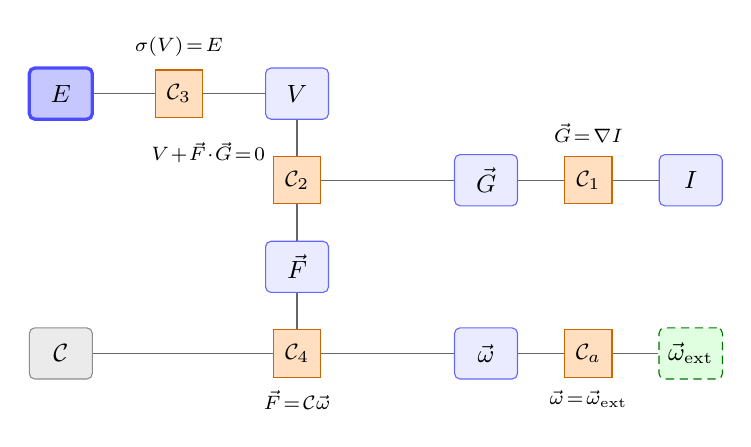
\begin{tikzpicture}[
  q/.style   = {rounded corners=2pt, draw=blue!60, fill=blue!8,
                minimum width=8mm, minimum height=6.5mm, font=\small},
  obs/.style = {q, draw=blue!70, fill=blue!22, very thick},
  con/.style = {q, draw=black!45, fill=black!8},
  c/.style   = {draw=orange!80!black, fill=orange!25,
                minimum width=6mm, minimum height=6mm, font=\footnotesize},
  ext/.style = {q, draw=green!45!black, fill=green!12, densely dashed},
  e/.style   = {draw=black!60, line width=0.5pt}]

% --- quantities -------------------------------------------------------
\node[obs] (E)  at (0,2.2)    {$E$};
\node[q]   (V)  at (3.0,2.2)  {$\Vmap$};
\node[q]   (G)  at (5.4,1.1)  {$\Gmap$};
\node[q]   (I)  at (8.0,1.1)  {$\Imap$};
\node[q]   (F)  at (3.0,0)    {$\Fmap$};
\node[con] (C)  at (0,-1.1)   {$\Cmat$};
\node[q]   (W)  at (5.4,-1.1) {$\wvec$};
\node[ext] (X)  at (8.0,-1.1) {$\wvec_{\text{ext}}$};

% --- costs ------------------------------------------------------------
\node[c] (c3) at (1.5,2.2)  {$\mathcal{C}_3$};
\node[c] (c2) at (3.0,1.1)  {$\mathcal{C}_2$};
\node[c] (c1) at (6.7,1.1)  {$\mathcal{C}_1$};
\node[c] (c4) at (3.0,-1.1) {$\mathcal{C}_4$};
\node[c] (ca) at (6.7,-1.1) {$\mathcal{C}_a$};

% --- edges ------------------------------------------------------------
\draw[e] (E)--(c3);   \draw[e] (c3)--(V);
\draw[e] (V)--(c2);   \draw[e] (c2)--(G);  \draw[e] (c2)--(F);
\draw[e] (G)--(c1);   \draw[e] (c1)--(I);
\draw[e] (F)--(c4);   \draw[e] (c4)--(W);  \draw[e] (C)--(c4);
\draw[e] (W)--(ca);   \draw[e] (ca)--(X);

% --- annotations ------------------------------------------------------
\node[font=\scriptsize, anchor=south] at (1.5,2.55) {$\sigma(\Vmap)\!=\!E$};
\node[font=\scriptsize, anchor=east]  at (2.72,1.45)
      {$\Vmap\!+\!\Fmap\!\cdot\!\Gmap\!=\!0$};
\node[font=\scriptsize, anchor=south] at (6.7,1.45) {$\Gmap\!=\!\nabla\Imap$};
\node[font=\scriptsize, anchor=north] at (3.0,-1.45) {$\Fmap\!=\!\Cmat\wvec$};
\node[font=\scriptsize, anchor=north] at (6.7,-1.45)
      {$\wvec\!=\!\wvec_{\text{ext}}$};
\end{tikzpicture}}
\caption{The model as an energy-based graphical model: quantities (rounded) are
related by costs (orange). Only the event map $E$ is observed (shaded) and
$\Cmat$ is a constant of the camera; $\Imap$, $\Gmap$, $\Fmap$ and $\wvec$ are
all inferred. $\mathcal{C}_1$--$\mathcal{C}_4$ are the relations of
Sec.~\ref{sec:model}. The anchoring cost $\mathcal{C}_a$ (dashed) is absent from
the model as published; Sec.~\ref{sec:scale} shows it is the condition under
which the rest works, and that $\wvec_{\text{ext}}$ can come either from a
gyroscope or from the events themselves.}
\label{fig:model}
\end{figure}

\subsection{Quantities and constraints}
\label{sec:model}

\subsubsection{Input}
An event camera pixel fires an event $e_k=(x_k,y_k,t_k,p_k)$ as soon as the
logarithmic intensity it observes has changed by a contrast threshold $\theta$
since the last event at that pixel~\cite{lichtsteiner2008}:
\begin{equation}
p_k = \begin{cases}
+1 & \text{if } \Delta \log \Imap(x_k,y_k,t_k) > \theta,\\
-1 & \text{if } \Delta \log \Imap(x_k,y_k,t_k) < -\theta .
\end{cases}
\end{equation}
Events are accumulated over a short window of duration $\Delta t$ into an
\emph{event frame}, the per-pixel signed event count
\begin{equation}
E(x,y) \;=\; \sum_{t_k \in [t, t+\Delta t)} p_k \, \delta(x-x_k)\,\delta(y-y_k),
\label{eq:eventframe}
\end{equation}
which is a direct correlate of the temporal derivative of the (log) intensity.
Both formulations use a scalar map $\Vmap \approx \partial \Imap/\partial t$
derived from~\eqref{eq:eventframe} as the \emph{only} input to the network. In
what follows $\Imap$ always denotes log-intensity, as is standard for event
cameras.

\subsubsection{Quantities}
The world is modelled as a static scene observed by a camera that is fixed in
position but free to rotate. Besides $\Vmap$, the model carries the
log-intensity map $\Imap$, its spatial gradient $\Gmap$, the optical flow
$\Fmap$, and the camera's angular velocity $\wvec\in\mathbb{R}^3$ --- the only
non-retinotopic quantity in the network. A constant map $\Cmat$ encodes the
camera geometry.

\subsubsection{Constraints}
Three relations tie these quantities together. The first is the optical-flow
constraint equation~\cite{horn1981}, which follows from assuming that intensity
is only transported in the image and not created or destroyed,
$\mathrm{d}\Imap/\mathrm{d}t = 0$:
\begin{equation}
\Vmap_{x,y} + \Fmap_{x,y}\cdot\Gmap_{x,y} \;=\; 0 .
\label{eq:ofce}
\end{equation}
The second is the definition of the gradient, discretised with forward
differences,
\begin{equation}
\Gmap_{x,y} \;=\; \nabla \Imap_{x,y}
 \;=\; \big(\Imap_{x+1,y}-\Imap_{x,y},\; \Imap_{x,y+1}-\Imap_{x,y}\big)^{\!\top}.
\label{eq:spatial}
\end{equation}
The third states that the flow induced by a pure rotation is, at every pixel, a
linear function of $\wvec$,
\begin{equation}
\Fmap_{x,y} \;=\; \Cmat_{x,y}\,\wvec ,
\label{eq:kin}
\end{equation}
with the $2\times3$ kinematic matrix obtained by differentiating the projection
of a rotating 3-D point~\cite{martel2019thesis}
\begin{equation}
\Cmat_{x,y} =
\begin{pmatrix}
 x'y' & -(x'^2+1) & y' \\[2pt]
 y'^2+1 & -x'y' & -x'
\end{pmatrix},
\label{eq:cmat}
\end{equation}
where $(x',y')$ are the normalised image coordinates of pixel $(x,y)$. Notably
$\Cmat_{x,y}$ does not depend on scene depth: rotational flow carries no
structure information, which is what makes the purely rotational model
self-contained.

\subsubsection{Underdetermination of the individual constraints}
Each constraint on its own is too weak to invert.
Equation~\eqref{eq:ofce} is one scalar equation in the four unknowns
$(\Fmap_{x,y},\Gmap_{x,y})$: given $\Vmap$ and $\Gmap$, the admissible $\Fmap$
form a line perpendicular to $\Gmap$ --- the aperture problem.
Equation~\eqref{eq:spatial} does not constrain $\Imap$ at all in the direction
of a constant offset, and $\Cmat_{x,y}$ in~\eqref{eq:kin} has rank~2 with kernel
spanned by $(x',y',1)^{\!\top}$, so a single flow vector leaves a whole line of
admissible $\wvec$. Only when all three are imposed simultaneously, over all
pixels, does a solution become determined. There is no feed-forward order in
which $\Imap$, $\Gmap$, $\Fmap$ and $\wvec$ can be computed from $\Vmap$; the
interpretation has to be found by iterating the constraints against each other.

\subsubsection{Scale ambiguity}
\label{sec:beta}
One degeneracy survives even the joint problem. For any $\beta\neq 0$ the
substitution
\begin{equation}
(\Imap,\Gmap,\Fmap,\wvec) \;\longmapsto\;
 (\beta\Imap,\;\beta\Gmap,\;\Fmap/\beta,\;\wvec/\beta)
\label{eq:beta}
\end{equation}
leaves \eqref{eq:ofce}--\eqref{eq:kin} satisfied identically. From a single
input frame it is therefore impossible to tell a slowly moving high-contrast
scene from a quickly moving low-contrast one, and since $\beta$ may be negative,
not even the sign of $\wvec$ is determined. Cook \emph{et al.} note that in
practice the ambiguity is resolved arbitrarily on the first frame by the random
initialisation and then held roughly constant by warm-starting each frame from
the previous converged state~\cite{cook2011}. As Sec.~\ref{sec:experiments}
shows, this is exactly where the method is fragile in a tracking setting.

\subsection{Variant I: Sequential Relaxation (Cook \emph{et al.})}
\label{sec:cook}

Cook \emph{et al.}~\cite{cook2011} derive the updates from a single recipe: to
update a map from one relation, assume the other maps in that relation are
correct, compute the \emph{candidate} map --- the closest map to the current one
that would satisfy the relation --- and take a small step of size $\delta$
towards it. This is a relaxation method applied to local constraints rather than
to a boundary-constrained differential equation.

For the nonlinear relation~\eqref{eq:ofce} the candidate is not unique, so the
constraint is turned into the quadratic error
$Q_{\Vmap,\Gmap}(\Fmap_{x,y}) = (\Vmap_{x,y}+\Fmap_{x,y}\cdot\Gmap_{x,y})^2$ and
a gradient step is taken,
\begin{equation}
\Fmap_{x,y} \leftarrow \Fmap_{x,y}
 - 2\,\delta_{\Vmap\!\Fmap\!\Gmap}\,
   (\Vmap_{x,y}+\Fmap_{x,y}\cdot\Gmap_{x,y})\,\Gmap_{x,y},
\label{eq:cook_ofce}
\end{equation}
and symmetrically for $\Gmap$. For the linear relations the candidate is
explicit. From~\eqref{eq:spatial},
$\Gmap_{x,y}\leftarrow(1-\delta_{I\!G})\Gmap_{x,y}+\delta_{I\!G}\nabla
\Imap_{x,y}$; in the opposite direction a change of $\Imap_{x,y}$ also affects
the gradients at the neighbours $(x\!-\!1,y)$ and $(x,y\!-\!1)$, so the residual
$\Psi=\Gmap-\nabla\Imap$ is differenced back,
$\hat\Psi^{(x)}_{x,y}=\Psi^{(x)}_{x,y}-\Psi^{(x)}_{x-1,y}$ (and analogously in
$y$), giving
\begin{equation}
\Imap_{x,y} \leftarrow \Imap_{x,y}
  - \delta_{G\!I}\big(\hat\Psi^{(x)}_{x,y}+\hat\Psi^{(y)}_{x,y}\big),
\label{eq:cook_poisson}
\end{equation}
a discrete Poisson step. Finally $\Fmap$ is blended towards $\Cmat\wvec$, and
$\wvec$ is obtained by a linear least-squares fit over the whole flow field,
which aggregates every pixel's weak opinion into one estimate. Cook stores
$\Imap$ on a $(H\!+\!1)\times(W\!+\!1)$ grid so that forward differences yield a
full $H\times W$ gradient.

The updates are applied \textbf{sequentially}: each map is written immediately,
so later updates within the same sweep already see the new values. This is a
Gauss--Seidel scheme, and the result consequently depends on the order in which
the relations are visited --- an order the paper does not fix.

\subsection{Variant II: Energy-Based Message Passing (Martel)}
\label{sec:martel}

Martel~\cite{martel2019thesis,martel2015relational} recasts the same system in a
\emph{quantity-centric} framework. A model is a bipartite graph whose nodes are
visual quantities and whose factors are explicit energy functions, in the spirit
of a factor graph~\cite{kschischang2001}. For the rotational model the total energy is
the sum of the four costs
\begin{align}
\mathcal{C}_{\text{tot}} = \sum_{x,y} \Big[ &
  \|\nabla \Imap_{x,y}-\Gmap_{x,y}\|^2
+ (\Vmap_{x,y}+\Fmap_{x,y}\cdot\Gmap_{x,y})^2 \nonumber\\
&+ (\sigma(\Vmap_{x,y})-E_{x,y})^2
+ \|\Fmap_{x,y}-\Cmat_{x,y}\wvec\|^2 \Big],
\label{eq:energy}
\end{align}
where the third term makes the event map $E$ an explicit quantity of the model,
related to $\Vmap$ through the sensor's level-crossing nonlinearity $\sigma$
rather than being identified with it.

Inference minimises~\eqref{eq:energy} greedily by message passing
(Algorithm~6.5 of~\cite{martel2019thesis}) in two phases per iteration. In
\emph{Phase~1} every quantity sends its current value to the costs it
participates in, and each cost computes its partial derivative with respect to
each of its quantities. In \emph{Phase~2} the costs send those derivatives back
and every quantity updates. Because the gradient operator is linear, a quantity
touched by several costs simply sums the messages it receives; e.g.\ $\Gmap$
receives contributions from both the spatial and the flow-constraint cost.
Nonlinear relations use gradient steps as in~\eqref{eq:cook_ofce}, whereas linear
relations admit a closed-form optimum and are updated by blending towards it. For
the angular velocity, setting $\partial \mathcal{C}/\partial\wvec = 0$ yields the
normal equations $M\wvec^\star = v$ with
\begin{equation}
M=\sum_{x,y}\Cmat_{x,y}^{\!\top}\Cmat_{x,y}, \qquad
v=\sum_{x,y}\Cmat_{x,y}^{\!\top}\Fmap_{x,y},
\label{eq:normaleq}
\end{equation}
and the update $\wvec \leftarrow \wvec - \eta(\wvec - M^{-1}v)$. Since $M$
depends only on the pixel grid and the intrinsics, $M^{-1}$ is a $3\times3$
matrix that can be precomputed once.

The decisive difference to Cook is that Phase~2 happens \textbf{simultaneously}:
all messages are computed from one common snapshot before anything is written.
This is a Jacobi scheme. It removes the dependence on update order and is the
property that makes the algorithm parallelisable and portable to
cellular-processor hardware, which is the thesis' motivation for it. The price
is paid in propagation: because every message is computed from a frozen
snapshot, information crosses one relation per iteration, whereas the sequential
scheme carries it across the whole network within a single sweep. The effect is
directly visible in Sec.~\ref{sec:converge}. Jacobi is also less forgiving of an
inconsistent starting state (Sec.~\ref{sec:implementation}). The thesis also derives extensions of the same
model --- a persistent world map, a stereo variant, and fusion with an inertial
measurement unit --- the last of which introduces a fourth cost pulling $\wvec$
towards an externally measured angular velocity. We implement this IMU fusion,
and then generalise it: the same cost accepts any external estimate of $\wvec$,
and we show in Sec.~\ref{sec:scale} that the gyroscope can be removed from it
altogether.

Table~\ref{tab:variants} summarises the comparison.

\begin{table}[!t]
\renewcommand{\arraystretch}{1.25}
\caption{The Two Formulations at a Glance}
\label{tab:variants}
\centering
\footnotesize
\begin{tabular}{@{}lll@{}}
\toprule
 & \textbf{Cook \emph{et al.}}~\cite{cook2011} & \textbf{Martel}~\cite{martel2019thesis} \\
\midrule
Framing      & interacting maps          & energy-based graph \\
Update order & sequential (Gauss--Seidel)& simultaneous (Jacobi) \\
Derivation   & candidate map + step      & $\partial\mathcal{C}/\partial q$ + step \\
Input        & $\Vmap$ (binned events)   & $E$, linked to $\Vmap$ by $\sigma$ \\
Flow model   & $\Fmap = m_{32}(\wvec\times \Cmat)$ & $\Fmap = \Cmat_{x,y}\wvec$ \\
$\wvec$ from $\Fmap$ & least squares on lines & normal equations~\eqref{eq:normaleq} \\
Extensions   & --- & persistence, stereo, IMU \\
\bottomrule
\end{tabular}
\end{table}

\subsection{Resolving the Scale Ambiguity}
\label{sec:scale}

Neither scheme removes the $\beta$-ambiguity of~\eqref{eq:beta}, because it is a
property of the constraints and not of the solver. Any remedy must therefore come
from outside them, in the form of a quantity that is stated in absolute units.
The thesis' own remedy is the IMU cost mentioned above: a gyroscope measures
$\wvec$ directly, so adding a term
\begin{equation}
\mathcal{C}_{\text{anchor}} \;=\; \|\wvec - \wvec_{\text{ext}}\|^2,
\qquad \wvec_{\text{ext}} = \wvec_{\text{gyro}}
\label{eq:anchorcost}
\end{equation}
pins down both scale and sign. We implement this first, and it works
(Sec.~\ref{sec:experiments}). It is, however, an unsatisfying answer to a
question posed by a vision system: the quantity the network cannot determine is
supplied by a second sensor rather than recovered from the data.

The observation this report builds on is that $\wvec_{\text{ext}}$
in~\eqref{eq:anchorcost} need not come from a sensor at all. Any estimator whose
objective is \emph{not} invariant under the rescaling~\eqref{eq:beta} can occupy
the same place in the graph.

Contrast maximization~\cite{gallego2018cmax} offers the same anchor from the
events alone. Under a candidate angular velocity $\wvec$, each event is warped to
a common reference time $t_{\text{ref}}$ along the trajectory the hypothesis
implies,
\begin{equation}
\vec{p}_k' \;=\; \vec{p}_k + \big(\wvec\,(t_k-t_{\text{ref}})\big)\times\vec{p}_k ,
\label{eq:warp}
\end{equation}
with $\vec{p}_k$ the bearing vector of event $k$. The warped events are
accumulated into the image of warped events (IWE), and $\wvec$ is chosen to
maximise its contrast, here the variance
\begin{equation}
\wvec^\star = \arg\max_{\wvec}\ \operatorname{Var}\!\big[\mathrm{IWE}(\wvec)\big].
\label{eq:cmax}
\end{equation}
The IWE is sharpest at the true motion and blurs when the hypothesis is wrong in
\emph{either} direction or magnitude. Objective~\eqref{eq:cmax} is therefore
\emph{not} invariant under the rescaling~\eqref{eq:beta}, which is precisely the
property the three constraints lack. Setting
$\wvec_{\text{ext}} = \wvec^\star$ in~\eqref{eq:anchorcost} therefore turns the
IMU cost into a sensor-free one, without changing anything else in the model.
Two ways of coupling the estimator to the message passing are described in
Sec.~\ref{sec:coupling} and compared in Sec.~\ref{sec:experiments}.


\section{Implementation}
\label{sec:implementation}

The system is implemented in Python with NumPy. All map updates are expressed as
whole-array operations, so a message-passing iteration costs a handful of vector
operations over the $180\times240$ sensor and no per-pixel loop is ever executed.

\subsection{Software Structure and Data Path}

The code is organised so that the two formulations share everything except the
solver: one module converts events into input frames, one builds the kinematic
matrix, one holds each network, one implements the contrast-maximization
estimator, and one drives the experiments. Any difference in output between the
two formulations is therefore attributable to the solver alone.

Events are read from the text format of~\cite{mueggler2017} and accumulated per
window into the signed-count image~\eqref{eq:eventframe}, which is then clipped
to $\pm c$ and divided by $c$, giving $\Vmap \in [-1,1]$. This is the standard
event-frame representation~\cite{gallego2022survey}. The accumulation window
$\Delta t$ serves simultaneously as the input window and as the time step
relating the network's internal $R$ (rad/frame) to the reported
$\wvec = R/\Delta t$ (rad/s).

Lens distortion can be removed at either end of this path, and both routes are
implemented. The first rectifies the event coordinates before accumulation and
leaves the kinematic matrix in its ideal pinhole form~\eqref{eq:cmat}. The second
keeps the events in their native pixel coordinates and moves the lens into the
geometry instead: $\Cmat_{x,y}$ is built from the true undistorted normalised
coordinates of each physical pixel and post-multiplied by the analytic Jacobian
$J_D$ of the distortion map, so that the predicted flow is expressed in
distorted-pixel units,
\begin{equation}
\Cmat_{x,y} \;=\; \operatorname{diag}(f_x,f_y)\; J_D(x',y')\; A(x',y'),
\label{eq:cdist}
\end{equation}
with $A$ the matrix of~\eqref{eq:cmat}. The second route avoids re-quantising
rectified sub-pixel coordinates onto the pixel grid during accumulation, and it
performed better in our experiments; it is used for every result reported below.
Sec.~\ref{sec:experiments} reports the comparison between the two.

Because both formulations assume a rotation-only observer, evaluation segments
are restricted to intervals in which this holds. A selection pass
slides a window over the gyroscope record and flags intervals of low angular
velocity variance; the selected segments span roughly a factor of five in
rotation speed, which turns out to matter (Sec.~\ref{sec:experiments}).

\subsection{The Two Networks}

Both networks are driven by the \emph{same} kinematic matrix~\eqref{eq:cmat} and
the same input frames, so that any difference in their output is attributable to
the update scheme alone rather than to the camera model. The Cook network applies
its updates in place, in a fixed order, and stores $\Imap$ on the
$(H\!+\!1)\times(W\!+\!1)$ grid of~\cite{cook2011}. The Martel network is built
from \texttt{Quantity} and \texttt{Cost} objects that mirror
Algorithm~6.5 directly: each cost implements a single method that reads the
current values and adds its contribution to the gradient accumulator of every
quantity it touches, and the solver only alternates the two phases. Adding a
relation therefore means adding one class and nothing else, which is how both
the anchoring cost and the contrast-maximization cost were introduced without
modifying the solver.

Two implementation decisions were necessary and are not stated in either source.
First, the simultaneous scheme requires a \emph{mutually consistent} initial
state: if $\wvec$ is initialised from a known value but $\Fmap$ is left at zero,
the kinematics cost sees a large residual and drives $\wvec$ to zero within a few
iterations, before the flow constraint has built any structure. Initialising
$\Fmap = \Cmat\wvec$ removes the problem entirely. Second, the flow-constraint
gradient in~\eqref{eq:cook_ofce} grows cubically when $|\Fmap|$ and $|\Gmap|$ are
both large, so it is clipped per pixel, and each quantity is clipped to a fixed
range after every iteration. These bounds are not inert: at high rotation speed
$\Gmap$ reaches its limit on real data, for the reason given in
Sec.~\ref{sec:cmax_exp}. They do not, however, affect the angular velocity ---
widening them by a factor of twenty changes the reported error by less than
$0.05^\circ$/s --- so they bound the maps without shaping the result we measure.

\subsection{Coupling Contrast Maximization to the Network}
\label{sec:coupling}

The estimator of Sec.~\ref{sec:scale} is used with a fixed-time window equal to
one frame, the reference time at the window midpoint, a linear warp, the variance
objective, and a warm start from the previous frame's estimate; it returns
$\wvec$ in rad/s in the camera body frame, the same convention as the network's
$R = \wvec\Delta t$. Two couplings to the message passing were implemented. They
differ in \emph{where} the contrast optimisation happens relative to the
relaxation loop, and consequently in what determines $\wvec$. The first reuses
the anchoring cost~\eqref{eq:anchorcost} unchanged and only substitutes its
target, so it is the gyroscope-anchored model with one sensor swapped for an
estimator; the second replaces the update rule for $\wvec$ entirely.

\subsubsection{Per-frame anchor}
The first (\texttt{CMax-anchor}) treats contrast maximization as an external
measurement. Once per frame, before any relaxation, the estimator is run to
convergence on that frame's events, giving $\wvec_{\text{cmax}}$. The anchoring
cost of Sec.~\ref{sec:scale} then contributes
\begin{equation}
\Delta \wvec \;=\; \delta_{\text{anchor}}\,
  \big(\wvec - \wvec_{\text{cmax}}\big)
\label{eq:anchor}
\end{equation}
at \emph{every} one of the iterations of that frame, alongside all the other
costs. The kinematics cost continues to update $\wvec$ from the flow field as
in~\eqref{eq:normaleq}. The angular velocity is therefore determined jointly by
the anchor and by the network, and the two can disagree. Because the estimator is
called once per frame and its gradient is not needed, the optimisation uses a
derivative-free simplex search on the blurred IWE.

\subsubsection{Interleaved update}
The second (\texttt{CMax-inloop}) removes the separation between the two
optimisations. The anchoring cost is dropped, and the kinematics cost is
restricted to propagating $\wvec$ into the flow field --- it still enforces
$\Fmap \leftarrow \Cmat\wvec$ but no longer updates $\wvec$ itself. In its place,
a single gradient-\emph{ascent} step on the contrast objective is taken once per
message-passing iteration,
\begin{equation}
\wvec \;\leftarrow\; \wvec \;+\; \lambda\,
  \frac{\partial}{\partial \wvec}\operatorname{Var}\!\big[\mathrm{IWE}(\wvec)\big],
\label{eq:inloop}
\end{equation}
so that the contrast optimisation and the relaxation of the maps advance
together rather than one after the other. This requires the analytic gradient of
the objective with respect to $\wvec$, obtained by scattering the derivatives of
the bilinear voting kernel into three images and differentiating the variance;
we verified it against finite differences. In this variant $\wvec$ is driven by
contrast maximization \emph{alone}: the maps receive it but never correct it.

The step size $\lambda$ in~\eqref{eq:inloop} is the one parameter without a
natural scale, since the gradient grows with the square of the number of events
in the window and therefore varies between sequences. We use a fixed
$\lambda = 10^{-4}$, which is stable over the datasets considered; an order of
magnitude larger diverges. Sec.~\ref{sec:experiments} shows that the difference
between the two couplings is almost entirely a difference in how the
\emph{magnitude} of $\wvec$ is determined, which is what one would expect from
the fact that only the first lets the kinematic constraint act on it.

\subsection{Deviations From the Published Descriptions}
\label{sec:deviations}

Neither source is complete enough to be implemented without choices. We list
ours explicitly, since some of them affect the comparison.

\begin{enumerate}
\item \textbf{Shared camera model.} Cook expresses the flow relation as
  $\Fmap = m_{32}(\wvec\times\Cmat)$ with $\Cmat$ a map of unit ray directions.
  We use the kinematic matrix~\eqref{eq:cmat} for \emph{both} networks. The two
  express the same geometry, and sharing it isolates the update scheme as the
  only difference.
\item \textbf{Angular velocity from flow.} Cook minimises the point-to-line
  distance between $\wvec$ and the family of rotations compatible with each flow
  vector; we use the normal equations~\eqref{eq:normaleq} in both networks.
\item \textbf{The event cost is omitted.} The term $(\sigma(\Vmap)-E)^2$
  of~\eqref{eq:energy} is not implemented: $\Vmap$ is identified with the
  normalised event frame rather than inferred from $E$ through the sensor
  nonlinearity. $\Vmap$ is therefore treated as observed, as in~\cite{cook2011}.
\item \textbf{Intensity update.} We implement
  $\Imap \leftarrow \Imap - \eta\operatorname{div}(\Gmap-\nabla \Imap)$ in both
  networks, i.e.\ Cook's~\eqref{eq:cook_poisson}, omitting the additional
  shrinkage term of the thesis' iterative form. The frequency-domain variant is
  not implemented.
\item \textbf{Step sizes.} Neither source reports the values of the relaxation
  step sizes. Ours were tuned by grid search (Table~\ref{tab:params}) and are
  examined in Sec.~\ref{sec:experiments}.
\end{enumerate}

\begin{table}[!t]
\renewcommand{\arraystretch}{1.2}
\caption{Adopted Parameters. \textnormal{Every result in this report uses these
values. $\delta_{F\!R}$ and $\delta_{\text{anchor}}$ were changed from the
$0.30$/$0.50$ and $0.30$ we began with, on the evidence of
Sec.~\ref{sec:sensitivity}; the sweep there varies each parameter from those
original values, so its highlighted row is not this configuration.}}
\label{tab:params}
\centering
\footnotesize
\begin{tabular}{@{}llcc@{}}
\toprule
Symbol & Relation & Cook & Martel \\
\midrule
$\delta_{\Vmap\!\Fmap\!\Gmap}$ & flow constraint~\eqref{eq:ofce} & 0.08 & 0.12 \\
$\delta_{I\!G}$ & $\Gmap$ from $\Imap$ & 0.12 & 0.10 \\
$\delta_{G\!I}$ & $\Imap$ from $\Gmap$ & 0.08 & 0.05 \\
$\delta_{R\!F}$ & $\Fmap$ from $\wvec$ & 0.03 & 0.05 \\
$\delta_{F\!R}$ & $\wvec$ from $\Fmap$ & 0.10 & 0.10 \\
$\delta_{\text{anchor}}$ & external $\wvec$ anchor~\eqref{eq:anchorcost} & --- & 0.50 \\
\midrule
\multicolumn{2}{@{}l}{iterations per frame} & \multicolumn{2}{c}{75} \\
\multicolumn{2}{@{}l}{window $\Delta t$} & \multicolumn{2}{c}{20\,ms} \\
\bottomrule
\end{tabular}
\end{table}

\subsection{Evaluation Harness}

A single code path produces every number in this report. A run is described by a
configuration object naming the dataset, the segment, the model and the
parameters; the harness then iterates over frames and writes per-frame estimates,
a summary and a tracking plot. Five models are evaluated, forming the progression
of Sec.~\ref{sec:scale}: the two pure-vision networks \texttt{cook} and
\texttt{thesis}; the gyroscope-anchored \texttt{thesis+IMU}; and the two
contrast-anchored variants of Sec.~\ref{sec:coupling}.

The two data sources play strictly separate roles. The gyroscope (\texttt{imu.txt})
is a \emph{model input}: it supplies the anchor target of \texttt{thesis+IMU} at
every iteration, and the warm start $R_0 = \wvec_{\text{gyro}}\Delta t$ of the
first frame, which \emph{every} model shares so that all are compared from an
identical initial state. No model is therefore entirely gyroscope-free; the
contrast-anchored variants differ in not using it inside the loop. The Vicon
record (\texttt{groundtruth.txt}) is the \emph{scoring reference}, obtained by
differencing consecutive orientations in the body frame,
$\Delta R = R_1^{\!\top}R_2$. Because the two come from different instruments,
scoring the gyroscope-anchored model this way is not circular; comparing it
against the gyroscope itself would be, and we never do.

The width of the differencing bracket matters more than it appears. Over a
single 20\,ms window the reference is dominated by pose noise: the gyroscope
scores $8$--$25^\circ$/s against it depending on the segment, so the metric
cannot resolve anything better than that regardless of the model. All results
below use a $\pm50$\,ms bracket, and every table reports the gyroscope's own
error against the same reference as an explicit noise floor.

Each frame is scored by the error $\|\wvec_{\text{est}}-\wvec_{\text{ref}}\|$ in
$^\circ$/s, the angle between the two vectors, and the scale factor
$\beta = \|\wvec_{\text{ref}}\| / \|\wvec_{\text{est}}\|$. The last is reported
separately throughout, because Sec.~\ref{sec:beta} predicts that the direction
and the magnitude of $\wvec$ fail independently, and they do.

Finally, $\wvec$ is \emph{recurrent}. It is initialised once before the first
frame and is never overwritten afterwards; each frame starts from the previous
frame's converged state, as in~\cite{cook2011}. No per-frame ground-truth
re-anchoring is used anywhere, so drift over a segment is fully visible.

\subsection{Development and Validation}

\subsubsection{Working with a language model}
The repository was written with the assistance of a large language model, and
since the practice is now common but rarely described, it is worth stating how.
We did not ask for an implementation of a method by name; the model has no
reliable knowledge of either source, and asking would have invited it to
reconstruct something plausible instead of what the papers specify. Instead we
supplied the source material --- the two papers, the relevant dissertation
chapter, and the dataset's file format --- and asked for a skeleton: the module
layout, the event-loading path, and class stubs for the two networks with the
update rules transcribed from the numbered equations. That skeleton was
produced quickly and was a reasonable starting point, which is where most of the
time saved was saved.

It was not, however, correct. The failure mode we encountered was consistent:
code that was structurally sound and superficially faithful, but that silently
substituted a plausible variant for what the text actually says --- a
centred difference where the paper specifies a forward difference, a symmetric
update where the paper's is asymmetric, a normalisation the paper does not have.
None of these produce errors; they produce slightly wrong answers. Our working
rule became that every generated update rule was checked line by line against the
equation it claimed to implement, and that anything not traceable to a numbered
equation was treated as our own design decision and documented as such
(Sec.~\ref{sec:deviations}). The model was also useful in the opposite
direction, as a reader: asking it to explain a derivation step, or to say what a
piece of our own code computed, caught several errors of ours. What it could not
do was tell us whether a result was right, which is what the validation below is
for.

\subsubsection{Layered validation}
The system was built in layers, each validated before the next was added: the
Cook network, then the Martel network, then the anchoring cost, then distortion
handling, then contrast maximization. Because the network's output is a single
3-vector that is hard to attribute to any one component, we relied on checks that
isolate components rather than on end-to-end accuracy alone. The distortion
geometry was verified against \texttt{cv2.projectPoints} and by a round-trip
test, and the two distortion routes were shown to agree on a fixed-rotation warp
to sub-pixel accuracy with the network removed
(Sec.~\ref{sec:experiments}). The analytic gradient of the contrast objective was
checked against finite differences. The contrast-maximization front-end was
validated against \emph{both} the gyroscope and Vicon before being connected to
the network at all, so that a later failure could be attributed to the coupling
rather than to the estimator.

One methodological lesson is worth recording, because it shaped the protocol of
Sec.~\ref{sec:experiments}: conclusions drawn from a single short segment did not
survive. A configuration that appeared clearly best on a few frames of one
medium-speed segment behaved qualitatively differently on a faster one. All
results below are therefore reported over multiple segments spanning a range of
rotation speeds, and never as a single aggregate number.


\section{Experiments}
\label{sec:experiments}

\subsection{Protocol}
\label{sec:protocol}

We evaluate on three rotation sequences of the Event-Camera
Dataset~\cite{mueggler2017}, recorded with a DAVIS240C ($240\times180$) that
provides events, a gyroscope and Vicon poses simultaneously, and on two synthetic
sequences from ECRot~\cite{guo2024cmaxslam}, rendered with a model of the same
sensor. Table~\ref{tab:datasets} lists them.

The synthetic camera is an \emph{idealised} DAVIS240C, and the difference is
worth stating because it bears on Sec.~\ref{sec:distortion}. It shares the
resolution and, to within half a percent, the focal length of the real sensor
($f = 200$ against $199.1$/$198.8$\,px), but its principal point sits at the
exact image centre where the real one is offset by $(12.2, 20.7)$\,px, and it
carries no lens distortion at all against $k_1 = -0.37$ for the real camera.
Each sequence is processed with its own calibration throughout, so the
distortion-aware kinematic matrix~\eqref{eq:cdist} reduces to the ideal pinhole
form on the synthetic data.

One exclusion is worth stating. \texttt{shapes\_rotation} is not used: its scene
contains a few isolated shapes on a blank background, and both formulations
require the dense spatial gradient that the flow constraint acts on.

\texttt{dynamic\_rotation} is included with a caveat. Part of its scene --- a
person --- can move independently of the camera, which the model of
Sec.~\ref{sec:model} cannot represent: it explains all image motion as
ego-rotation. Over the segment reported here the person is largely stationary,
so the assumption is approximately met, but it is not guaranteed as it is
elsewhere. We report the sequence because the reconstructed maps remain
qualitatively correct on it, and read its angular-velocity numbers as an
indication of robustness rather than as a clean measurement.

The synthetic sequences depict busy scenes --- a street with pedestrians, a
cyclist --- but are nonetheless static in the sense the model requires: they are
rendered by rotating a virtual camera inside a fixed high-resolution panorama,
so the depicted people are frozen and all image motion is ego-motion. We
verified this on the sequences themselves: at the closest revisit of a camera
orientation, $5$\,s apart, the two frames differ only by a uniform,
edge-aligned residual consistent with the residual $1.8^\circ$ of
misalignment, with no localised difference anywhere in the scene. The contrast
with \texttt{dynamic\_rotation} is therefore one of scene \emph{motion}, not
scene content.

The two synthetic sequences earn their place on grounds of measurement precision
rather than realism. Their bags carry the simulator's own angular velocity, so
the reference needs no differencing and their simulated gyroscope agrees with it
to $0.10^\circ$/s, against $6$--$9^\circ$/s for the real sequences. They can
therefore resolve differences between models that the real data cannot, at the
cost of lacking both real sensor noise and a real lens.
Usefully, the two were generated along the \emph{same} camera trajectory --- we
verified that their pose records agree to $5\times10^{-7}$ in quaternion
components --- over different scenes, and differ by a factor of three in event
density ($4.6$ against $1.6$ events per pixel per frame). They therefore form a
controlled pair, varying scene content with the motion held fixed, which
Sec.~\ref{sec:speed} uses to rule out one explanation of the magnitude error.

Each segment is $150$ frames of $\Delta t = 20$\,ms, i.e.\ three seconds of
continuous tracking --- long enough for drift to appear, which shorter
evaluations hide. The segment reported per sequence is the one of median
rotation speed, chosen on that criterion alone and not on any model's error.
Because Sec.~\ref{sec:speed} finds that accuracy depends systematically on
rotation speed, reporting a single segment per sequence would otherwise amount
to an undeclared choice of operating point; Fig.~\ref{fig:beta_speed} therefore
shows every segment.

Segments are additionally required to hold $\wvec$ roughly constant, and it is
worth being clear that this is a constraint of the \emph{measurement}, not of
the model: the constraints of Sec.~\ref{sec:model} hold instantaneously for any
$\wvec$, changing or not. It matters because of how the reference is obtained.
On the real sequences Vicon records \emph{orientations}, so an angular velocity
has to be recovered by differencing two of them, and that difference is only
meaningful if $\wvec$ is approximately constant across the bracket. The
synthetic sequences are exempt --- their reference is the simulator's own
angular velocity at every instant --- which is one reason their noise floor is
sixty times lower. A reference obtained by fitting a rotation spline through the
poses and differentiating it analytically would remove this restriction and
allow longer or more varied segments; we did not implement one.

\texttt{dynamic\_rotation} is the one exception, and deliberately so. Selecting
by rotation speed there would ignore the property that makes the sequence
awkward in the first place, and in fact selects a segment in which the person
stands up and walks across the field of view. We instead report the segment in
which the scene is most nearly static --- the person seated, with the camera
providing essentially all of the image motion --- since that is what decides
whether the model's assumptions hold. The criterion is different from the other
sequences and we state it rather than fold it in.

Unless stated otherwise all runs use the parameters of
Table~\ref{tab:params}, $75$ iterations per frame, and the distortion-aware
kinematic matrix~\eqref{eq:cdist}. Every model is warm-started identically and
$\wvec$ is recurrent thereafter, so the numbers below include accumulated drift.

Two of the six step sizes, $\delta_{F\!R}$ and $\delta_{\text{anchor}}$, were
chosen by the sweep of Sec.~\ref{sec:sensitivity}, which also verified that both
sit at an interior optimum on the real sequences rather than at the edge of the
range searched. The remaining four were set by hand early on and were never
optimised, so the configuration should be read as tuned in two dimensions, not
as an optimum of the whole parameter space.

\begin{table}[!t]
\renewcommand{\arraystretch}{1.2}
\caption{Evaluation Sequences}
\label{tab:datasets}
\centering
\footnotesize
\begin{tabular}{@{}llccc@{}}
\toprule
Sequence & Seg. & $\|\wvec\|$ & Floor & Source \\
 & & (rad/s) & ($^\circ$/s) & \\
\midrule
\texttt{boxes\_rotation}   & seg\_B & 0.88 & 6.7 & ECD~\cite{mueggler2017} \\
\texttt{poster\_rotation}  & seg\_C & 0.91 & 9.0 & ECD~\cite{mueggler2017} \\
\texttt{dynamic\_rotation} & seg\_D & 0.74 & 8.3 & ECD~\cite{mueggler2017} \\
\texttt{bicycle}           & seg\_A & 1.32 & 0.10 & ECRot~\cite{guo2024cmaxslam} \\
\texttt{street}            & seg\_A & 1.32 & 0.10 & ECRot~\cite{guo2024cmaxslam} \\
\bottomrule
\end{tabular}
\end{table}

\subsection{Results}
\label{sec:mainresults}

Table~\ref{tab:main} reports every model on the five sequences at the
configuration selected in Sec.~\ref{sec:sensitivity}, namely
$\delta_{F\!R} = 0.1$ and $\delta_{\text{anchor}} = 0.5$. Both differ from the
values we began with, and both were chosen by the sweep of
Table~\ref{tab:sweep}. Since that sweep runs on the same sequences reported
here, the choice deserves a word. What justifies it is not the size of the
improvement but its consistency: each parameter moves the error in the same
direction on all five sequences \emph{independently}, including the synthetic
one, whose scene, sensor model and noise characteristics differ from the other
two. A setting that helps on three unrelated sequences separately is a property
of the model rather than a fit to any one of them. Table~\ref{tab:sweep} reports
the full sweep from the original defaults, so the effect of the choice is
visible rather than absorbed.

The pattern is the same on all five sequences and is stated here once.

Without an absolute reference, neither formulation is usable. Direction errors of
$73$--$82^\circ$ over three seconds mean the recovered axis carries essentially
no information about the true one, and total errors of $53$--$75^\circ$/s exceed
the rotation being measured.

Adding an anchor changes the picture entirely, and most of what the anchor
provides does not depend on where it comes from. Both anchored models recover the
rotation axis to $9$--$13^\circ$ on the real sequences and to $1$--$2^\circ$ on
the synthetic one, against $73$--$82^\circ$ without an anchor, and both bring
$\beta$ to within $14\%$ of unity against a collapse of two orders of magnitude.
Measured against what the anchor is for, the two are interchangeable.

Measured on total error they are not quite. The gyroscope is consistently ahead
of the contrast estimate, by $2.6^\circ$/s on \texttt{boxes}, $2.5$ on
\texttt{poster} and $0.8$ on the synthetic sequence. The gap is real and we do
not claim parity: an inertial measurement of $\wvec$ remains a better anchor than
an estimate inferred from the events. What the comparison does establish is that
the estimate is close enough to stand in for it --- within $1$--$3^\circ$/s of a
dedicated sensor, on a quantity the network cannot determine at all on its own,
using nothing but the data already being processed.

Two further points are visible in Table~\ref{tab:main}. On both real sequences
the gyroscope-anchored model scores \emph{better than the gyroscope itself}
against the independent Vicon reference ($6.5$ against $6.7$, and $8.9$ against
$9.0^\circ$/s). Since the reference is a third instrument, this cannot be an
artefact of the comparison: the visual constraints are filtering the inertial
signal rather than merely being overridden by it, which is the behaviour the
interacting-maps architecture is meant to produce. And the two update schemes
remain indistinguishable throughout --- \texttt{cook} and \texttt{thesis} differ
by a few percent and fail in the same way on every sequence. What separates
Gauss--Seidel from Jacobi is not accuracy but the rate at which they converge,
which Sec.~\ref{sec:converge} shows directly.

Figure~\ref{fig:tracking} shows what the aggregate numbers describe. The
anchored network follows the reference through a full reversal of $\omega_x$ and
the onset of $\omega_z$, with a residual that is visible but bounded. The
unanchored network is the flat trace: having settled on one scale in the first
few frames, it stays there, reproducing neither the reversal nor the magnitude.
It is not tracking poorly --- it is not tracking.

\begin{figure}[!t]
\centering
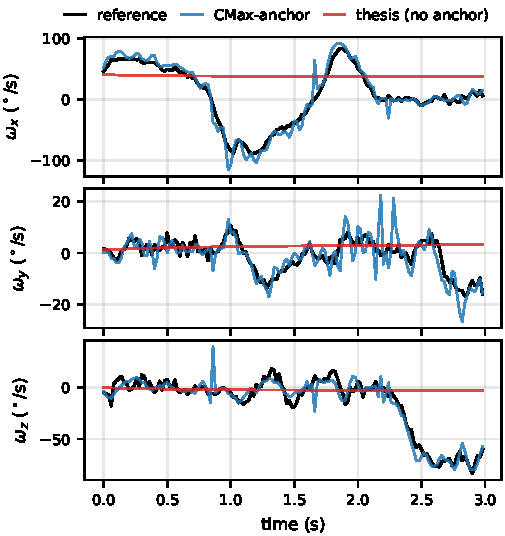
\includegraphics[width=\columnwidth]{fig_tracking}
\caption{Angular velocity over the three-second \texttt{poster} segment,
component-wise, against the Vicon reference. The contrast-anchored network
tracks; the same network without an anchor settles on an arbitrary constant and
stays there, which is the $\beta$-ambiguity of~\eqref{eq:beta} resolving itself
once and then persisting through the recurrent state.}
\label{fig:tracking}
\end{figure}

Figure~\ref{fig:maps} shows the remaining quantities, which the angular-velocity
metrics do not capture. The intensity map is recovered well enough for the scene
to be recognised although $\Imap$ is never observed, the gradient map
concentrates on scene edges, and the flow field varies smoothly across the image
as a pure rotation requires. This is also the evidence for the caveat attached to
\texttt{dynamic\_rotation} in Sec.~\ref{sec:protocol}: the reconstruction there
is of the same quality as on the static sequences even though the scene contains
a person, which is why we report the sequence rather than exclude it.

The reconstruction is not, however, uniform along a track, and the figure shows
a favourable moment. Following $\Imap$ frame by frame on the anchored model, its
standard deviation varies between $0.03$ and $1.59$ over the three seconds of
\texttt{poster}, with the excursions concentrated at the peaks of the rotation;
the same network without an anchor stays between $0.02$ and $0.05$ throughout.
During those excursions the map loses its structure and the gradient map reaches
the bound of Sec.~\ref{sec:implementation}. The angular velocity is unaffected
--- the errors reported here are computed over the whole track, excursions
included --- but the visual interpretation and the quantity we score are not
equally reliable at all times, and only the latter has been measured
systematically.

\begin{figure*}[!t]
\centering
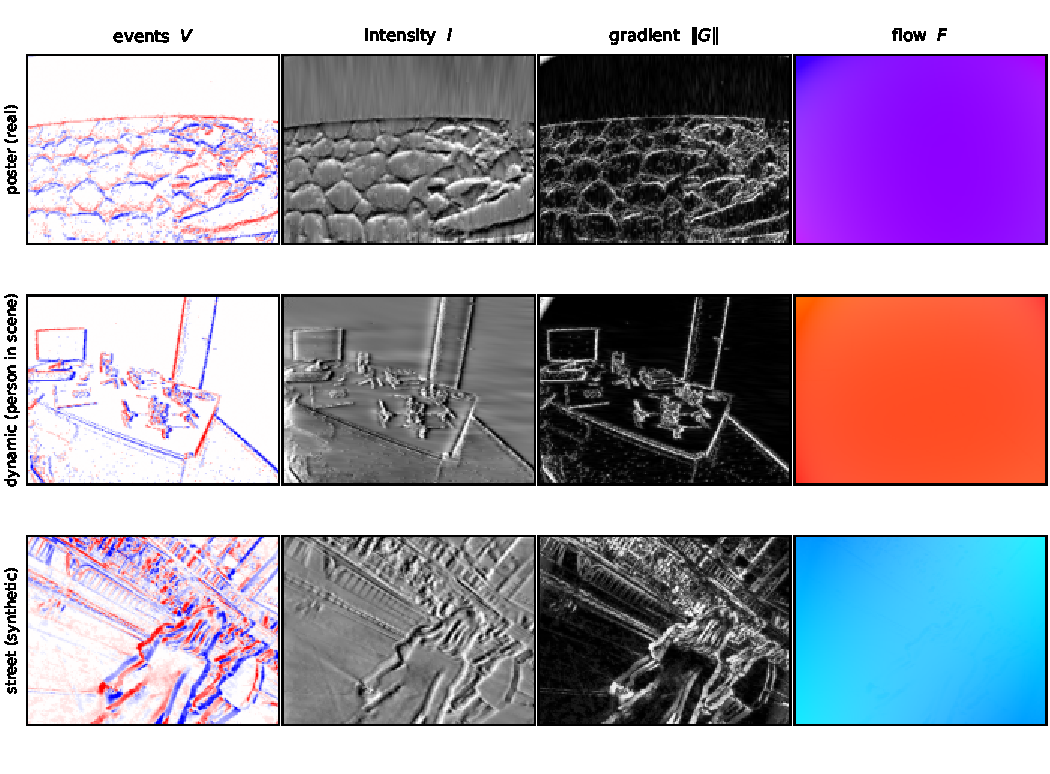
\includegraphics[width=\textwidth]{fig_maps}
\caption{Jointly inferred quantities after $40$ frames, for two real sequences
and one synthetic one. Only $\Vmap$ is observed; $\Imap$, $\Gmap$ and $\Fmap$
are inferred. Flow is shown as hue for direction and saturation for magnitude.
The middle row is the \texttt{dynamic\_rotation} segment of
Sec.~\ref{sec:protocol}, in which a person is present in the scene but seated;
the camera is pointed at the desk for the frame shown.}
\label{fig:maps}
\end{figure*}

\begin{table}[!t]
\renewcommand{\arraystretch}{1.15}
\caption{Main Results. \textnormal{150 frames ($3$\,s) per sequence, default
parameters, scored against the $\pm50$\,ms reference. The gyroscope's own error
against that reference is the noise floor of each comparison. The last row of
each block is not a model: it is the gyroscope reading scored against the same
reference as everything above it, and it bounds what any estimate could
demonstrate here.}}
\label{tab:main}
\centering
\footnotesize
\begin{tabular}{@{}llrrr@{}}
\toprule
Sequence & Model & err ($^\circ$/s) & dir ($^\circ$) & $\beta$ \\
\midrule
\multirow{6}{*}{\shortstack[l]{\texttt{boxes}\\$0.88$\,rad/s}}
 & \texttt{cook}        & 63.2 & 79.7 & 1.02 \\
 & \texttt{thesis}      & 57.4 & 79.5 & 1.31 \\
 & \texttt{thesis+IMU}  & \textbf{6.5} & \textbf{9.2} & \textbf{1.00} \\
 & \texttt{CMax-anchor} & 9.1 & 10.7 & 0.91 \\
 & \texttt{CMax-inloop} & 10.5 & 16.9 & 0.90 \\
 & \emph{gyro vs Vicon}  & \emph{6.7} & \emph{9.2} & --- \\
\midrule
\multirow{6}{*}{\shortstack[l]{\texttt{poster}\\$0.91$\,rad/s}}
 & \texttt{cook}        & 56.8 & 72.9 & 1.07 \\
 & \texttt{thesis}      & 53.2 & 73.1 & 1.35 \\
 & \texttt{thesis+IMU}  & \textbf{8.9} & \textbf{12.5} & \textbf{1.05} \\
 & \texttt{CMax-anchor} & 11.3 & 12.3 & 0.86 \\
 & \texttt{CMax-inloop} & 13.4 & 16.6 & 1.00 \\
 & \emph{gyro vs Vicon}  & \emph{9.0} & \emph{12.5} & --- \\
\midrule
\multirow{6}{*}{\shortstack[l]{\texttt{dynamic}\\$0.74$\,rad/s\\(person)}}
 & \texttt{cook}        & 50.5 & 91.0 & 1.08 \\
 & \texttt{thesis}      & 47.1 & 91.5 & 1.32 \\
 & \texttt{thesis+IMU}  & \textbf{8.0} & \textbf{12.1} & \textbf{1.01} \\
 & \texttt{CMax-anchor} & 10.5 & 13.0 & 0.89 \\
 & \texttt{CMax-inloop} & 11.5 & 14.2 & 1.01 \\
 & \emph{gyro vs Vicon}  & \emph{8.3} & \emph{12.1} & --- \\
\midrule
\multirow{6}{*}{\shortstack[l]{\texttt{bicycle}\\$1.32$\,rad/s\\(synthetic)}}
 & \texttt{cook}        & 74.9 & 82.2 & 209.9 \\
 & \texttt{thesis}      & 74.1 & 77.9 & 2.63 \\
 & \texttt{thesis+IMU}  & \textbf{6.5} & \textbf{1.1} & \textbf{1.09} \\
 & \texttt{CMax-anchor} & 7.3 & 1.9 & 1.10 \\
 & \texttt{CMax-inloop} & 48.8 & 25.9 & 1.09 \\
 & \emph{gyro vs Vicon}  & \emph{0.10} & \emph{0.06} & --- \\
\midrule
\multirow{6}{*}{\shortstack[l]{\texttt{street}\\$1.32$\,rad/s\\(synthetic)}}
 & \texttt{cook}        & 74.8 & 71.9 & 436.3 \\
 & \texttt{thesis}      & 74.8 & 79.6 & 2.50 \\
 & \texttt{thesis+IMU}  & \textbf{6.5} & \textbf{1.1} & \textbf{1.09} \\
 & \texttt{CMax-anchor} & 7.1 & 2.1 & 1.09 \\
 & \texttt{CMax-inloop} & 794.7 & 53.3 & 0.16 \\
 & \emph{gyro vs Vicon}  & \emph{0.10} & \emph{0.06} & --- \\
\bottomrule
\end{tabular}
\end{table}

The synthetic sequences deserve separate comment, because their reference is not
differenced at all. The ECRot bags record the simulator's own angular velocity,
so the reference is exact and the simulated gyroscope agrees with it to
$0.10^\circ$/s --- roughly seventy times below the errors being measured, and
sixty times better than the reference available on the real sequences. That lets
them answer a question the real data cannot: how much of the residual error
belongs to the model rather than to the reference. On the real sequences the
anchored models sit at the floor, so the question is unanswerable there; here it
is not, and the answer is that essentially all of it is the model's. The
anchored variants reach $6.5$ and $7.1$--$7.3^\circ$/s with the rotation axis
recovered to about $1$--$2^\circ$, and the remainder is almost entirely
magnitude error, $\beta \approx 1.09$.

The two sequences also agree with each other to within $0.2^\circ$/s and
$0.02$ in $\beta$ on every anchored model, despite differing threefold in event
density. Since they share a camera trajectory exactly, this is a direct
statement that the residual error depends on the motion and the model, not on
what the camera is looking at.

The same clarity applies to the failure case. Where the real sequences show the
pure-vision networks at $\beta \approx 1.0$--$1.4$ --- a plausible-looking scale
attached to a meaningless direction --- on the synthetic pair \texttt{cook}
settles at $\beta = 210$ and $436$, angular velocities more than two orders of
magnitude too small, while still producing a self-consistent set of maps. That
the same model reaches two such different scales on two sequences filmed along
the \emph{same} trajectory is the $\beta$-ambiguity in its purest form: the
constraint system is satisfied either way, and which scale it lands on is
arbitrary.

\subsection{The Scale Ambiguity in Practice}
\label{sec:beta_exp}

The three constraints of Sec.~\ref{sec:model} determine $\wvec$ only up to the
rescaling~\eqref{eq:beta}. Table~\ref{tab:anchor} shows what that costs on real
data. Without an absolute reference, neither formulation produces a usable
estimate over three seconds: direction errors of $72$--$100^\circ$ mean the
recovered axis carries essentially no information about the true one, and the
magnitude is worse still --- on the fastest segment the Cook network settles at
$\beta \approx 29$, i.e.\ an angular velocity too small by more than an order of
magnitude. This is not a tuning failure. It is the ambiguity resolving itself
arbitrarily, exactly as~\eqref{eq:beta} permits, and then being carried forward
by the recurrent state.

It is worth being precise about what does \emph{not} fix this. Every model in
Table~\ref{tab:anchor}, including the two pure-vision ones, is warm-started from
the gyroscope: $\wvec$ begins at the correct value on frame~0. That is
sufficient only for the first few frames. Once the relaxation is free to rescale
$\Gmap$ against $\Fmap$, nothing in the cost function prefers the initial scale
to any other, and the estimate leaves it. An absolute reference supplied
\emph{once} therefore does not anchor the model; it has to be present in the
cost that is minimised at every iteration.

Adding the gyroscope term~\eqref{eq:anchorcost} does exactly that, and the
failure disappears: the error falls by a factor of six to nine, direction error
from $72$--$100^\circ$ to $12$--$15^\circ$, and on the slowest segment $\beta$
returns to $1.00$. That segment also gives the clearest evidence that the
network contributes something of its own. The anchored model reaches
$5.44^\circ$/s against Vicon while the gyroscope that anchors it scores
$5.51^\circ$/s against the same reference: the fused estimate is \emph{closer to
ground truth than its own anchor}. Since the reference is a third instrument,
independent of both, this cannot be an artefact of the comparison. The margin is
narrow, but the same ordering appears on \texttt{boxes} ($6.47$ against $6.73$)
and \texttt{dynamic} ($8.04$ against $8.31$), so it is not a single accident.
The visual constraints are not merely being overridden by the gyroscope; they
are filtering it, which is the behaviour the interacting-maps architecture is
meant to produce.

\begin{table}[!t]
\renewcommand{\arraystretch}{1.15}
\caption{Effect of the Anchor. \textnormal{Poster sequence, three segments of
150 frames at the configuration of Table~\ref{tab:main}, scored against Vicon
($\pm50$\,ms). The gyroscope's own error against the same reference is the noise
floor of the comparison. This sequence is shown because it spans the widest
range of rotation speed of the three real ones; the same comparison on
\texttt{boxes} and \texttt{dynamic} gives the same ratios to within a factor of
$1.5$.}}
\label{tab:anchor}
\centering
\footnotesize
\begin{tabular}{@{}llrrr@{}}
\toprule
$\|\wvec\|$ & Model & err ($^\circ$/s) & dir ($^\circ$) & $\beta$ \\
\midrule
\multirow{6}{*}{$1.67$}
 & \texttt{cook}          &  94.3 &  82.6 & 148.1 \\
 & \texttt{thesis}        & 107.0 &  71.8 &  1.62 \\
 & \texttt{thesis+IMU}    &  11.8 &  14.6 &  1.07 \\
 & \texttt{CMax-anchor}   &  16.5 &  19.3 &  0.89 \\
 & \texttt{CMax-inloop}   &  24.0 &  34.0 &  0.77 \\
 & \emph{gyro vs Vicon}    & \emph{11.6} & \emph{14.8} & --- \\
\midrule
\multirow{6}{*}{$0.91$}
 & \texttt{cook}          &  56.8 &  72.9 &  1.07 \\
 & \texttt{thesis}        &  53.2 &  73.1 &  1.35 \\
 & \texttt{thesis+IMU}    &   8.9 &  12.5 &  1.05 \\
 & \texttt{CMax-anchor}   &  11.3 &  12.3 &  0.86 \\
 & \texttt{CMax-inloop}   &  13.4 &  16.6 &  1.00 \\
 & \emph{gyro vs Vicon}    & \emph{9.0} & \emph{12.5} & --- \\
\midrule
\multirow{6}{*}{$0.42$}
 & \texttt{cook}          &  44.7 & 100.2 &  0.55 \\
 & \texttt{thesis}        &  38.7 &  99.1 &  0.65 \\
 & \texttt{thesis+IMU}    &   5.4 &  13.5 &  1.00 \\
 & \texttt{CMax-anchor}   &   8.5 &  13.5 &  0.79 \\
 & \texttt{CMax-inloop}   &   8.9 &  14.3 &  0.80 \\
 & \emph{gyro vs Vicon}    & \emph{5.5} & \emph{13.6} & --- \\
\bottomrule
\end{tabular}
\end{table}

\subsection{Replacing the Gyroscope with Contrast Maximization}
\label{sec:cmax_exp}

The anchor of~\eqref{eq:anchorcost} does not have to be a measurement. Replacing
$\wvec_{\text{gyro}}$ by the contrast-maximization estimate leaves the model
otherwise untouched and removes the second sensor from the loop.

Compared at equal anchor weight, the substitution costs something, and it is
worth being exact about how much. Over the fourteen segments measured, the
gyroscope-anchored model is ahead of the contrast-anchored one by between
$0.4$ and $4.7^\circ$/s, typically by $1$--$3$. The gap is narrowest on the
synthetic sequences, where the reference is exact ($0.6$ and $0.8^\circ$/s), and
widest on the fastest real segment (Table~\ref{tab:anchor}: $16.5$ against
$11.8^\circ$/s at $1.67$\,rad/s). Set against $107^\circ$/s for the same network
unanchored, both recover the overwhelming majority of what an anchor provides;
between the two, an inertial measurement remains the better reference.

The comparison is only meaningful because both anchors carry the same weight,
and it is sensitive to that choice: at a weaker $\delta_{\text{anchor}}$ the two
move closer together, which would flatter the visual anchor rather than inform
about it. We therefore report both at the same value throughout, and note from
Table~\ref{tab:sweep} that the ordering is stable across every weight tested.

One apparent advantage of the contrast anchor does not survive tuning, and is
worth recording because it is the kind of result that would otherwise be reported
as a finding. At the original defaults its scale factor was $1.00$ on both real
sequences against $1.08$ and $1.16$ for the gyroscope, suggesting a visual anchor
free of the inertial one's bias. At the configuration of
Table~\ref{tab:main} the ordering reverses ($0.91$ and $0.86$ against $1.00$ and
$1.05$). Both anchors are biased, in opposite directions, by amounts comparable
to the difference between them; neither is systematically better on scale, and
the appearance that one was is an artefact of where the kinematic weight
happened to sit.

\subsubsection{The two couplings differ in how they fix the magnitude}
\texttt{CMax-anchor} has the lower direction error on every segment
($19.4$, $12.5$, $12.2^\circ$ against $34.0$, $16.6$, $14.3^\circ$). The
comparison of total error is less straightforward and illustrates why $\beta$ is
reported separately. On the fast segment \texttt{CMax-inloop} has the
\emph{lower} total error ($24.0$ vs $32.8^\circ$/s) despite nearly twice the
direction error, because the two estimators err in opposite directions in
magnitude --- $\beta = 0.77$ against $1.18$ --- and for
\texttt{CMax-inloop} the magnitude and direction errors partially cancel inside
the norm. Ranking on total error alone would select the worse estimator. The
difference between the couplings is therefore almost entirely a difference in
how $\|\wvec\|$ is determined, which is what Sec.~\ref{sec:coupling} predicts:
only \texttt{CMax-anchor} leaves the kinematic constraint acting on $\wvec$.

\subsubsection{Magnitude error is a property of the network, not of the anchor}
\label{sec:speed}
Pooling every segment of both real sequences, which spans
$\|\wvec\| = 0.42$ to $1.67$\,rad/s, makes the pattern unambiguous. For
\texttt{CMax-anchor} the scale factor is almost perfectly correlated with
rotation speed,
\begin{equation}
\operatorname{corr}\big(\|\wvec\|,\ \beta\big) = +0.96 \quad (n=7,\ p<0.001),
\label{eq:betacorr}
\end{equation}
rising monotonically from $\beta = 0.80$ at the slowest segment to $\beta = 1.18$
at the fastest --- from a $20\%$ overestimate to an $18\%$ underestimate of
$\|\wvec\|$. For \texttt{CMax-inloop} the same correlation is $-0.47$, which at
this sample size is not significant ($p \approx 0.3$) and is in any case of the
opposite sign: whatever governs its magnitude, it is not the same
speed-dependent shrinkage.

That contrast localises the mechanism. The two variants share the estimator, the
input, the camera model and the maps, and differ in exactly one respect: whether
the kinematic cost is allowed to update $\wvec$. The shrinkage appears only when
it is, so it is produced by the kinematic update fitting $\wvec$ to a flow field
that is systematically too slow. The gyroscope-anchored model shows the same
trend ($\beta = 1.00, 1.16, 1.33$ over the three poster segments of
Table~\ref{tab:anchor}), confirming that the effect belongs to the network and
not to any particular anchor.

Why the inferred flow is too small follows from the ambiguity itself. Equation
\eqref{eq:beta} leaves the split of the flow constraint between $\Fmap$ and
$\Gmap$ undetermined, and the relaxation resolves it from the data. The anchor
constrains $\wvec$ but nothing constrains that split, so the kinematic cost ---
which carries a larger step size than the anchor
(Table~\ref{tab:params}) --- pulls $\wvec$ towards whatever $\Fmap$ the visual
side has settled on, and that flow field is too slow.

One natural refinement of this account is that the split should depend on scene
contrast: a high-contrast scene drives $\Gmap$ up, so a correspondingly smaller
$\Fmap$ satisfies $\Vmap = -\Fmap\cdot\Gmap$ equally well. The two synthetic
sequences test exactly this and refute it. They were rendered along the
\emph{same} camera trajectory over different scenes and differ by a factor of
three in event density, yet at matched parameters they yield
$\beta = 1.480$ and $1.483$ --- indistinguishable. Scene content, at least as
event density varies it, does not set the magnitude error.

That leaves a difference we cannot presently explain. At
$\|\wvec\| = 1.32$\,rad/s both synthetic sequences give $\beta \approx 1.48$
where the trend of~\eqref{eq:betacorr} fitted to the real ones predicts
$\approx 1.10$. Whatever distinguishes them is shared by both synthetic
sequences and is not their scene, their event density or their rotation speed.
We report the discrepancy rather than resolve it.

We can rule out one candidate explanation. The value clipping of
Sec.~\ref{sec:implementation} is not responsible, although it is active: the
gradient map does reach its bound on the real sequences whenever the anchor
drives $\wvec$ to a large value. It is nonetheless not the cause, because
widening all three bounds by a factor of twenty changes the error by less than
$0.05^\circ$/s and $\beta$ by less than $0.002$ on every sequence. The saturation is
therefore a consequence of the same imbalance, not its origin, and the effect is
a property of the constraint system rather than of the safeguards around it.

The account above makes a testable prediction: if the shrinkage is produced by
the kinematic update out-weighting the anchor, then reducing $\delta_{F\!R}$
should weaken the dependence on speed, not merely shift it. Repeating the
seven-segment measurement at $\delta_{F\!R} = 0.1$ confirms this. The
correlation of~\eqref{eq:betacorr} falls from $+0.96$ to $+0.60$ --- no longer
significant at $n = 7$ --- and the spread of $\beta$ across the full range of
rotation speeds halves, from $0.80$--$1.18$ to $0.79$--$0.97$. The residual
$\beta < 1$ is a roughly constant offset rather than a trend. A single step size
in a cost the constraint system leaves undetermined therefore governs the entire
speed dependence, which is the strongest evidence we have that the mechanism is
the one proposed here.

A control supports the same conclusion. \texttt{CMax-inloop}, in which the
kinematic cost does not act on $\wvec$ at all, returns \emph{identical} results
at both configurations on every sequence for which both were run
(Table~\ref{tab:main}): neither $\delta_{F\!R}$ nor $\delta_{\text{anchor}}$
reaches it. The parameters act only through the paths the model says they do.

The two couplings therefore trade off along different axes.
\texttt{CMax-anchor} has the better direction estimate on every segment of both
sequences, but its magnitude degrades with speed. \texttt{CMax-inloop} keeps a
speed-independent magnitude and loses on direction. Which one has the lower
\emph{total} error consequently depends on the sequence, and on the fast
segments the ranking inverts purely because the two error components partially
cancel for one of them.

This reframes the fast-segment result. It is not a failure of contrast
maximization, which supplies an accurate magnitude there, but a limitation of
the relaxation that no anchor can repair.

\begin{figure}[!t]
\centering
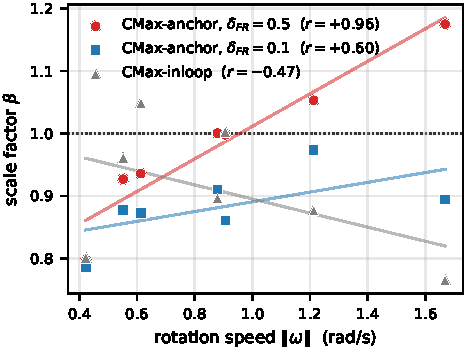
\includegraphics[width=\columnwidth]{fig_beta_speed}
\caption{Scale factor $\beta$ against mean rotation speed for every segment of
the two real sequences. \texttt{CMax-anchor} (in which the kinematic cost
updates $\wvec$) shows a strong speed dependence, $r = +0.96$;
\texttt{CMax-inloop} (in which it does not) shows no comparable trend,
$r = -0.47$, n.s. $\beta > 1$ means the magnitude is underestimated.}
\label{fig:beta_speed}
\end{figure}

\subsection{Convergence Within a Frame}
\label{sec:converge}

Everything above measures the state the network reaches after $75$ iterations.
How it gets there is worth showing, both because it is the mechanism the two
formulations actually differ in and because it is the clearest illustration of
what joint inference means here.

Figure~\ref{fig:converge} follows the intensity map through the iterations of a
single frame, with the network initialised from noise at that frame rather than
warm-started from the previous one, so that what is shown is what a single
$20$\,ms event map supports on its own. $\Imap$ is never observed; nevertheless
the scene assembles itself over a few tens of iterations, sharpening
monotonically to iteration $75$, by which point the signage in the scene can be
read. Nothing in the model computes $\Imap$ from $\Vmap$ --- it emerges from the
three constraints being applied against each other. In a running track each
frame starts from its predecessor's state instead, so this is the hardest case
rather than the typical one.

The two update schemes reach that state very differently. The sequential scheme
of Cook \emph{et al.} has recognisable structure after a \emph{single}
iteration, because each sub-update immediately sees the output of the one
before it, so information crosses the whole network within one sweep. The
simultaneous scheme is still noise at iterations one and three and only develops
structure by about ten, because every message is computed from a common snapshot
and therefore travels one relation per iteration. By iteration $75$ the two are
comparable, which is why they score alike in Table~\ref{tab:main}: the
difference between Gauss--Seidel and Jacobi in this model is one of convergence
rate, not of the solution reached.

Speed is not free. On the synthetic sequence the sequential scheme is also the
less stable of the two: it produces a good map at the first iterations and then
diverges, collapsing to an almost flat field by iteration ten, while all four
simultaneous variants converge normally on the same input. This is consistent
with the thesis' preference for the simultaneous scheme on grounds other than
accuracy.

\begin{figure*}[!t]
\centering
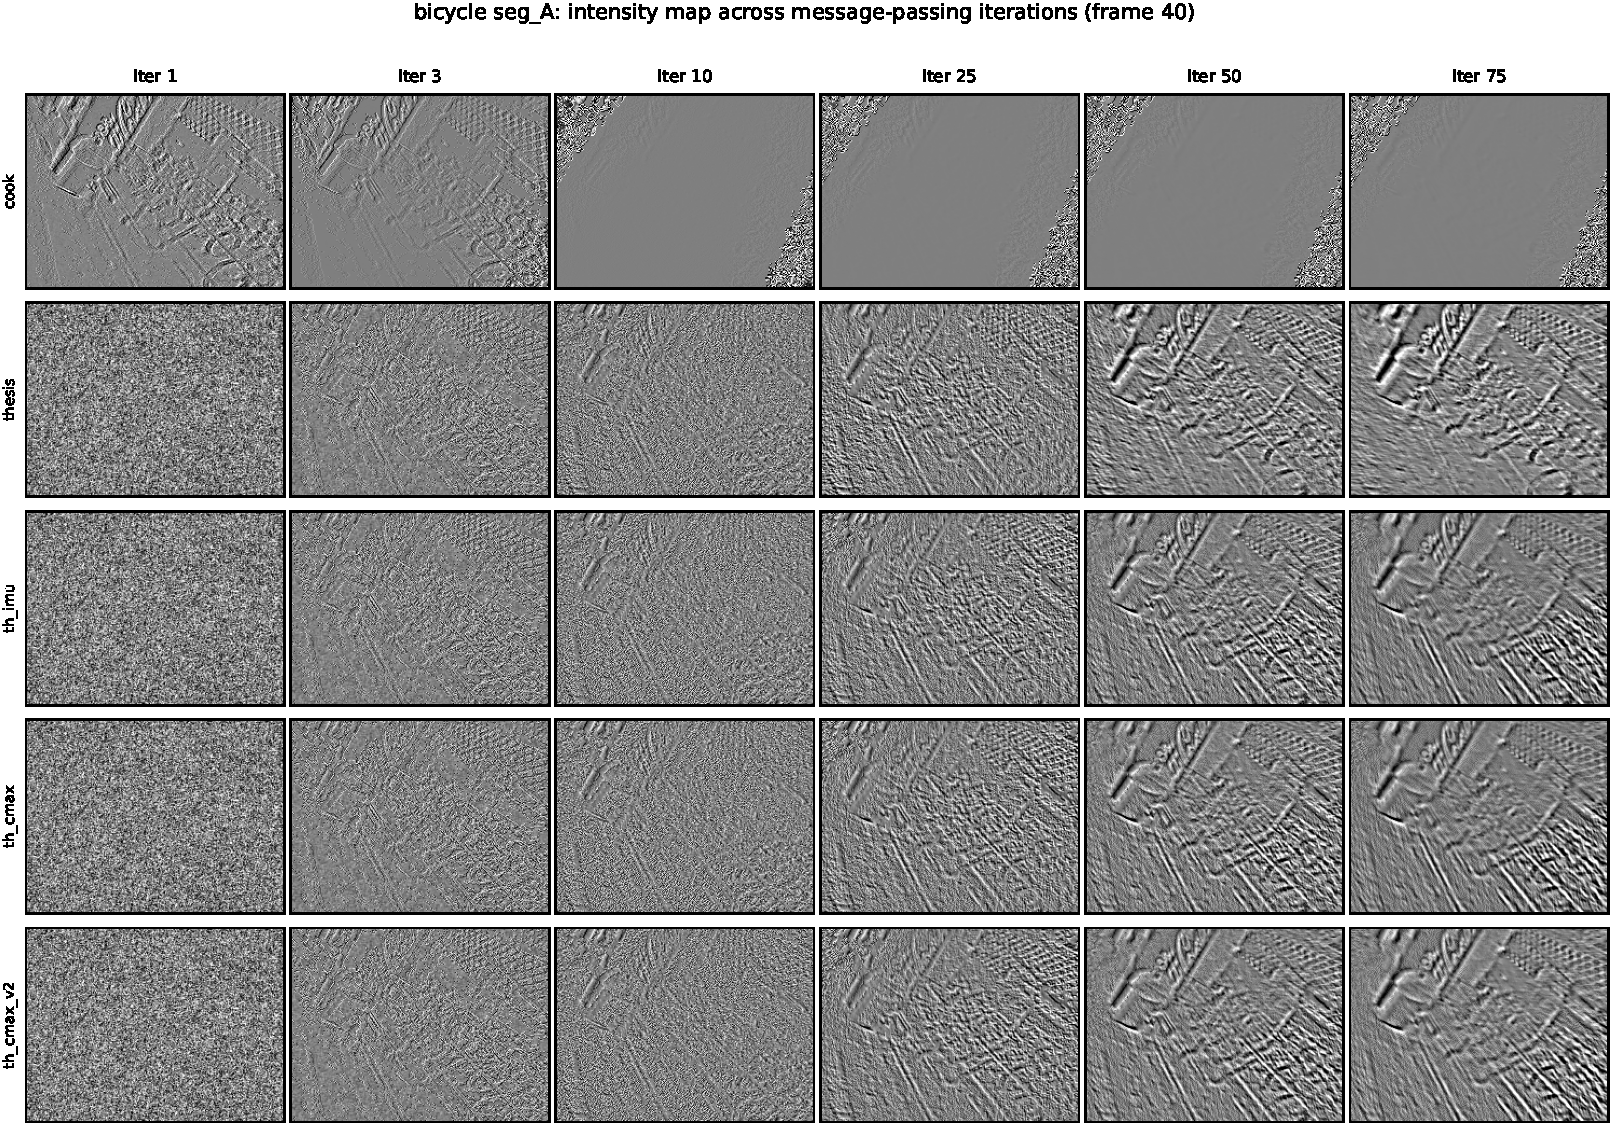
\includegraphics[width=\textwidth]{fig_converge_bicycle}
\caption{Intensity map across the message-passing iterations of a single frame
(\texttt{bicycle}, frame $40$). The network is initialised from noise at this
frame rather than warm-started from the preceding one, so the sequence shows
what one $20$\,ms event map alone supports; in a running track each frame would
instead begin from its predecessor's converged state. $\Imap$ is never observed.
The sequential scheme (top row) has structure after one iteration but diverges
by iteration ten on this sequence; the simultaneous variants develop structure
by iteration ten and sharpen to $75$, at which point the signage is legible. The
corresponding figure for \texttt{poster}, where the sequential scheme remains
stable, is in Appendix~\ref{app:converge}.}
\label{fig:converge}
\end{figure*}

\subsection{Handling Lens Distortion}
\label{sec:distortion}

The DAVIS240C lens is appreciably distorted ($k_1 = -0.37$), and
Sec.~\ref{sec:implementation} described two ways of accounting for it. Both are
correct as geometry; they differ in where the correction is applied, and that
turns out to matter for a reason unrelated to the geometry.

\subsubsection{The two routes describe the same lens}
Before comparing accuracy we verified that the distortion-aware kinematic
matrix~\eqref{eq:cdist}, which is our own derivation rather than something taken
from either source, encodes the lens correctly. Because the network's scale
ambiguity would confound any end-to-end comparison, the check is made with the
network removed, using contrast maximization as an independent estimator: one
path undistorts the events and warps them under a pinhole model, the other keeps
the events raw and carries the lens through the warp, as $\Cmat$ does. Three
checks agree. The forward distortion model matches \texttt{cv2.projectPoints} to
$2.8\times10^{-14}$\,px; undistortion and distortion compose to the identity to
$10^{-8}$\,px; and --- the decisive one --- at a fixed rotation, warping the
distortion-aware way and then undistorting the result lands on the pinhole warp
to $0.043$\,px, well below one pixel. The two routes are the same map.

\subsubsection{Why one is nevertheless better}
The difference is one of sampling, not geometry, and it is visible directly in
the input. \texttt{cv2.undistortPoints} returns sub-pixel float coordinates,
which the accumulation of~\eqref{eq:eventframe} must then bin onto the integer
pixel grid. Rectification compresses the periphery, so neighbouring events are
rounded onto the same pixel while others are left empty, and the resulting event
frame carries a concentric moir\'e pattern that is not present in the data
(Fig.~\ref{fig:distortion}). Over the same events, undistorting first reduces
the number of occupied pixels from $43.2$k to $33.7$k: roughly a fifth of the
spatial support of $\Vmap$ is lost to rounding. The spatial gradient $\Gmap$ is
computed by differencing neighbouring pixels of $\Imap$, so an artefact at
exactly that scale is the worst kind for this model.

Carrying the lens in $\Cmat$ avoids the resampling entirely: the events stay on
the pixels that produced them, and the distortion is applied to the
\emph{prediction} instead, where it costs nothing. We therefore use the
distortion-aware $\Cmat$ for every result in this report.

\begin{figure}[!t]
\centering
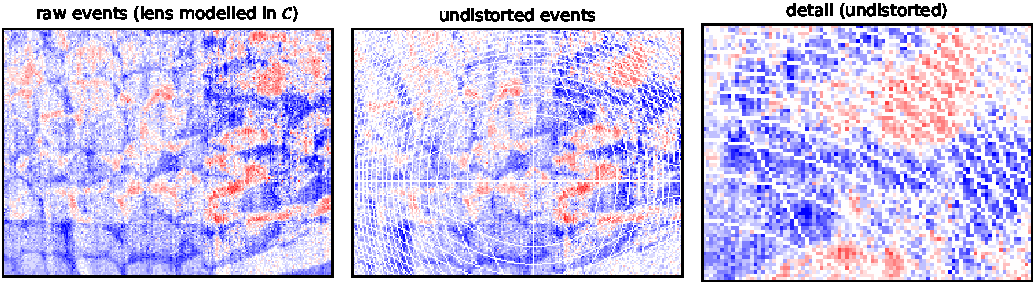
\includegraphics[width=\columnwidth]{fig_distortion}
\caption{Event frames over the same $200$\,ms of \texttt{poster}. Left: raw
events, with the lens carried by $\Cmat$~\eqref{eq:cdist}. Middle: the same
events after \texttt{cv2.undistortPoints}, showing the concentric moir\'e left
by re-quantising sub-pixel coordinates onto the pixel grid. Right: detail of the
periphery, where rectification compresses hardest and the artefact is strongest.
The pattern is a sampling artefact, not scene structure.}
\label{fig:distortion}
\end{figure}

\subsection{Sensitivity Analysis and Ablation}
\label{sec:sensitivity}

Table~\ref{tab:sweep} varies each parameter in turn from the configuration of
Table~\ref{tab:params}, on all five sequences. Two of the four sweeps are
informative, and one of them changes what we would recommend. Every trend below
holds on all five sequences independently, which is what makes them worth
reporting: the sequences differ in scene, in sensor (real against simulated), in
rotation speed by a factor of three and in event density by a factor of eight.

\subsubsection{Removing the anchor}
Setting $\delta_{\text{anchor}} = 0$ makes the anchoring
cost~\eqref{eq:anchorcost} contribute nothing, leaving the network exactly as
Cook and Martel specify it. This is the ablation of the fusion term, and because
the removed cost is the only place either anchor enters, it is the same model
for both. The error rises by a factor of $2.9$ to $6.4$ and the direction error
from $6$--$13^\circ$ to $73$--$92^\circ$. Nothing else in the sweep comes close
to this effect, which is the quantitative form of the argument in
Sec.~\ref{sec:beta_exp}: the anchor is not a refinement of the method but the
condition under which it works at all.

Over the range in Table~\ref{tab:sweep} the anchor weight is monotone ---
stronger is better, on every sequence, for \emph{both} anchors --- and $\beta$
approaches unity as it increases. That trend does not continue indefinitely:
raising $\delta_{\text{anchor}}$ to $0.7$ or $0.9$ is worse than $0.5$ on all
five sequences, so this parameter, too, has an interior optimum. The two anchors
also converge as the weight grows. At
$\delta_{\text{anchor}} = 0.1$ they differ by up to $1.4^\circ$/s; at $0.5$ they
agree to $0.5^\circ$/s or better on every sequence, and on the two synthetic
ones to $0.2^\circ$/s. The better the anchor is trusted, the less it matters
which one it is --- the clearest support we have for the claim that what the
model requires is an absolute reference, not specifically an inertial one.

\subsubsection{The kinematic weight}
The step size $\delta_{F\!R}$ of the kinematic update tests the mechanism
proposed in Sec.~\ref{sec:speed} directly. If the magnitude shrinkage is caused
by that update out-weighting the anchor, then $\delta_{F\!R}$ should control it
monotonically. It does, over essentially the whole admissible range: the update
is a blend $\wvec \leftarrow \wvec - \delta_{F\!R}(\wvec - \wvec^\star)$, so
$\delta_{F\!R} = 1$ would replace $\wvec$ by the flow-derived estimate outright,
and across $0.1$ to $0.9$ the scale factor rises without exception ---
$0.92 \rightarrow 1.07$ on \texttt{boxes}, $0.88 \rightarrow 1.06$ on
\texttt{poster}, and $1.15 \rightarrow 1.65$ on the synthetic sequence. The
error follows, most sharply where the shrinkage is largest: on the synthetic
sequence it runs from $10.4$ to $31.0^\circ$/s and the direction error from
$2.5$ to $8.1^\circ$. A parameter the constraint system treats as arbitrary
turns out to control the dominant error.

Extending the sweep below the smallest value in Table~\ref{tab:sweep} shows that
$\delta_{F\!R}$ has an optimum, and that where it lies depends on the data. On
the three real sequences $\delta_{F\!R} = 0.1$ is the best of every value tested:
going down to $0.05$ and $0.02$ makes the error worse again ($9.05 \rightarrow
9.34 \rightarrow 9.60^\circ$/s on \texttt{boxes}, and similarly on the other
two). On the two synthetic sequences it keeps improving, and steeply --- $7.30
\rightarrow 4.50 \rightarrow 2.83^\circ$/s on \texttt{bicycle}, with $\beta$
falling to $1.03$ and the direction error to $1.5^\circ$.

The split has a natural reading. Lowering $\delta_{F\!R}$ shifts authority over
$\wvec$ from the flow field to the anchor, so the best value should depend on
how good the anchor is. On the synthetic sequences the contrast estimate is very
accurate and trusting it further continues to pay; on real data it is noisier,
and past a point the flow field --- biased though it is --- carries information
the anchor does not. The optimal balance between a model's internal constraint
and its external reference is therefore a property of the data, not a constant
of the method, which is worth knowing for anyone tuning it on a new sequence.

\subsubsection{Iterations and window}
The remaining two parameters matter much less. Iterations per frame are
essentially irrelevant beyond $25$ --- across $25$ to $150$ the error varies by
under $0.7^\circ$/s on the real sequences and by $0.04^\circ$/s on the synthetic
one --- so the $50$--$75$ of~\cite{martel2019thesis} can be reduced threefold at
no cost. The accumulation window has a clear optimum at $20$\,ms on all five
sequences, degrading in both directions. The two directions fail differently:
$10$\,ms yields too few events per frame for a stable gradient, whereas
$50$\,ms yields a \emph{better} direction estimate on the synthetic sequence
($3.5$ against $6.0^\circ$) but a much worse magnitude ($\beta = 1.84$ against
$1.48$) --- more motion per window, and therefore more of the shrinkage of
Sec.~\ref{sec:speed}.

\begin{table*}[!t]
\renewcommand{\arraystretch}{1.15}
\caption{Sensitivity and Ablation, All Five Sequences. \textnormal{Each block
varies one parameter with all others held fixed, starting from the values we
began with (\textbf{bold}) rather than from the adopted configuration of
Table~\ref{tab:params} --- this is the sweep that led to the change, so it is
reported from its own starting point. Left number is the mean error in
$^\circ$/s, right is the mean direction error in degrees.
$\delta_{\text{anchor}}=0$ removes the anchoring cost entirely, so it is the
same model for both anchors and is listed once.}}
\label{tab:sweep}
\centering
\footnotesize
\begin{tabular}{@{}llrrrrrrrrrr@{}}
\toprule
& & \multicolumn{2}{c}{\texttt{boxes}} & \multicolumn{2}{c}{\texttt{poster}}
& \multicolumn{2}{c}{\texttt{dynamic}} & \multicolumn{2}{c}{\texttt{bicycle}}
& \multicolumn{2}{c}{\texttt{street}} \\
\cmidrule(lr){3-4}\cmidrule(lr){5-6}\cmidrule(lr){7-8}\cmidrule(lr){9-10}\cmidrule(lr){11-12}
& & err & dir & err & dir & err & dir & err & dir & err & dir \\
\midrule
\multicolumn{12}{@{}l}{\emph{anchor weight} $\delta_{\text{anchor}}$, contrast anchor}\\
& $0$ (abl.)     & 57.2 & 79.5 & 53.3 & 73.1 & 47.0 & 91.5 & 74.5 & 79.6 & 75.6 & 82.7 \\
& $0.1$          & 13.0 & 13.1 & 14.2 & 12.7 & 11.2 & 11.5 & 34.7 & 10.0 & 34.7 & 10.0 \\
& $\mathbf{0.3}$ & 10.5 & 10.4 & 11.4 & 12.5 & 10.0 & 12.1 & 25.6 &  6.0 & 25.5 &  6.0 \\
& $0.5$          &  9.7 & 10.5 & 10.2 & 12.5 &  9.5 & 12.5 & 20.5 &  4.5 & 20.3 &  4.6 \\
\midrule
\multicolumn{12}{@{}l}{\emph{anchor weight} $\delta_{\text{anchor}}$, gyroscope}\\
& $0.1$          & 11.6 &  9.5 & 13.9 & 10.8 & 10.6 & 10.1 & 34.6 &  9.7 & 34.6 &  9.7 \\
& $\mathbf{0.3}$ &  9.0 &  9.1 & 11.5 & 11.9 &  9.6 & 11.3 & 25.3 &  5.5 & 25.4 &  5.5 \\
& $0.5$          &  7.9 &  9.1 & 10.3 & 12.2 &  9.0 & 11.7 & 20.1 &  4.0 & 20.1 &  4.0 \\
\midrule
\multicolumn{12}{@{}l}{\emph{kinematic weight} $\delta_{F\!R}$}\\
& $0.1$          &  8.9 & 10.6 & 10.6 & 12.3 &  9.8 & 12.9 & 10.4 &  2.5 & 10.2 &  2.6 \\
& $0.3$          &  9.7 & 10.5 & 10.2 & 12.4 &  9.5 & 12.5 & 20.5 &  4.5 & 20.3 &  4.6 \\
& $\mathbf{0.5}$ & 10.5 & 10.4 & 11.4 & 12.5 & 10.0 & 12.1 & 25.6 &  6.0 & 25.5 &  6.0 \\
& $0.7$          & 11.1 & 10.5 & 12.4 & 12.6 & 10.4 & 11.8 & 28.8 &  7.2 & 28.7 &  7.2 \\
& $0.9$          & 11.6 & 11.1 & 13.0 & 12.6 & 10.7 & 11.6 & 31.0 &  8.1 & 30.9 &  8.1 \\
\midrule
\multicolumn{12}{@{}l}{\emph{iterations per frame}}\\
& $25$           & 10.5 & 12.2 & 10.6 & 12.3 &  9.0 & 11.0 & 25.7 &  6.1 & 25.5 &  6.1 \\
& $50$           & 10.3 & 10.7 & 11.1 & 12.5 &  9.6 & 11.5 & 25.6 &  6.0 & 25.5 &  6.0 \\
& $\mathbf{75}$  & 10.5 & 10.4 & 11.4 & 12.5 & 10.0 & 12.1 & 25.6 &  6.0 & 25.5 &  6.0 \\
& $150$          & 10.9 & 10.6 & 11.6 & 12.5 & 10.4 & 12.9 & 25.7 &  6.0 & 25.5 &  6.1 \\
\midrule
\multicolumn{12}{@{}l}{\emph{accumulation window} $\Delta t$}\\
& $10$\,ms          & 16.8 & 18.1 & 16.8 & 14.4 & 13.9 & 16.2 & 32.5 & 26.1 & 26.8 & 21.0 \\
& $\mathbf{20}$\,ms & 10.5 & 10.4 & 11.4 & 12.5 & 10.0 & 12.1 & 25.6 &  6.0 & 25.5 &  6.0 \\
& $50$\,ms          & 18.4 &  9.2 & 18.3 & 11.8 & 15.6 & 11.0 & 34.6 &  3.5 & 34.4 &  3.5 \\
\bottomrule
\end{tabular}
\end{table*}


\section{Conclusion}
\label{sec:conclusion}

We have re-implemented both published formulations of Interacting Maps --- the
sequential relaxation of Cook \emph{et al.} and the energy-based message passing
of Martel's dissertation --- on a shared camera model, data path and evaluation
harness, and evaluated them on five sequences against an independent reference.
To our knowledge no implementation of either was previously available.

The clearest result is negative and concerns the method as published. On
three-second tracks neither formulation produces a usable angular velocity:
direction errors of $73$--$91^\circ$ mean the recovered axis is uninformative,
and the magnitude can leave any plausible range entirely, reaching
$\beta = 432$ on one sequence while the maps remain mutually consistent. This is
not a tuning failure but the scale ambiguity of~\eqref{eq:beta} resolving itself
arbitrarily, and warm-starting from the correct value does not prevent it: the
estimate leaves the initial scale as soon as the relaxation is free to rescale
$\Gmap$ against $\Fmap$. The choice of update scheme is, by comparison,
immaterial --- Gauss--Seidel and Jacobi differ by a few percent and fail in the
same way.

What makes the method work is an absolute reference inside the cost that is
minimised at every iteration. Supplied by a gyroscope, as the thesis proposes,
it reduces the error by three to nine times and brings the direction error to
$1$--$13^\circ$. Our main positive result is that this reference need not be a
measurement: a contrast-maximization estimate computed from the same events
occupies the same place in the model and comes within $0.6$--$2.6^\circ$/s of
the inertial anchor on the five reported sequences, without a second sensor.
Over the wider set of fourteen segments the gap reaches $4.7^\circ$/s at the
highest rotation speeds. We do not claim parity --- the gyroscope remains ahead
throughout --- but the gap is small next to what the anchor buys. Notably, on three of the five sequences the
fused estimate is closer to the Vicon reference than the gyroscope that anchors
it, so the visual constraints are filtering the inertial signal rather than
merely being overridden by it.

We also characterised the residual error. It is almost entirely a magnitude
error, it grows with rotation speed ($r = +0.96$ over seven segments), and it is
produced by the kinematic cost fitting $\wvec$ to a flow field that the visual
side systematically underestimates: it appears only when that cost updates
$\wvec$, and its step size controls it monotonically across the whole admissible
range. Two candidate explanations were tested and rejected --- value clipping,
which fewer than $0.04\%$ of pixels reach, and scene content, which two
synthetic sequences sharing a trajectory but differing threefold in event
density leave unchanged. Why both synthetic sequences sit well above the trend
fitted to the real ones remains open.

Three practical findings are worth recording. Lens distortion should be carried
in the kinematic matrix rather than removed from the events, not for geometric
reasons --- the two routes agree to $0.043$\,px --- but because rectifying event
coordinates and re-binning them destroys about a fifth of the spatial support of
$\Vmap$ at exactly the scale the gradient operates on. Twenty-five iterations
per frame suffice where the thesis uses $50$--$75$. And the tighter of the two
contrast-maximization couplings, in which a gradient step on the contrast
replaces the update rule for $\wvec$, is not robust: its step size scales with
the square of the event count and it diverged outright on the densest sequence.

\subsection*{Outlook}

The most immediate opportunity follows from the sensitivity analysis. The two
parameters that matter, $\delta_{F\!R}$ and $\delta_{\text{anchor}}$, were found
by grid search, yet the network already computes the quantities that indicate
how they should be set --- the per-relation residuals. Adapting them online from
those residuals, rather than fixing them in advance, would remove the one part
of this system that currently requires a human.

A more substantial extension is to stop treating contrast maximization as an
external anchor. At present the events are used twice: once through $\Vmap$ and
once, independently, inside the estimator. Optimising the contrast of the warped
events \emph{jointly} with the map relaxation --- rather than solving one and
injecting the answer into the other --- would make motion compensation part of
the network instead of a component bolted onto it, and is the natural way to
express contrast maximization in the quantity-centric framework of
Sec.~\ref{sec:martel}. The failure of the tighter coupling reported here
suggests this is worth doing carefully rather than by simply interleaving the
two optimisations.

Finally, the model itself invites extension in the direction both sources
indicate: adding a persistent scene map so that information survives beyond one
frame, and relaxing the pure-rotation assumption, which would require depth to
enter the network and would make the sequences we had to exclude admissible.


\appendices
\section{Inferred Maps for Every Sequence}
\label{app:maps}

Figure~\ref{fig:appendix} shows the full set of inferred quantities for each of
the five sequences of Table~\ref{tab:main}, on the same segments and at the same
configuration, after $40$ frames. Only the event map is observed. The angular
velocity is the quantity we evaluate numerically because it is the one for which
an independent reference exists, but it is not the only output of the model, and
the maps are worth inspecting directly: the intensity map is recovered well
enough for every scene to be recognised despite never being measured, the
gradient concentrates on scene edges, and the flow field varies smoothly as a
pure rotation requires. The reconstruction quality is visibly similar across
real and synthetic data and is not obviously worse on \texttt{dynamic}, whose
scene contains a person.

These are single frames, chosen at the same point of each track, and as
Sec.~\ref{sec:mainresults} notes the reconstruction is not uniform in time: at
the peaks of the rotation the intensity map loses structure for a few tenths of
a second before recovering. The panels above are representative of the majority
of each track but not of its worst moments.

\begin{figure*}[!t]
\centering
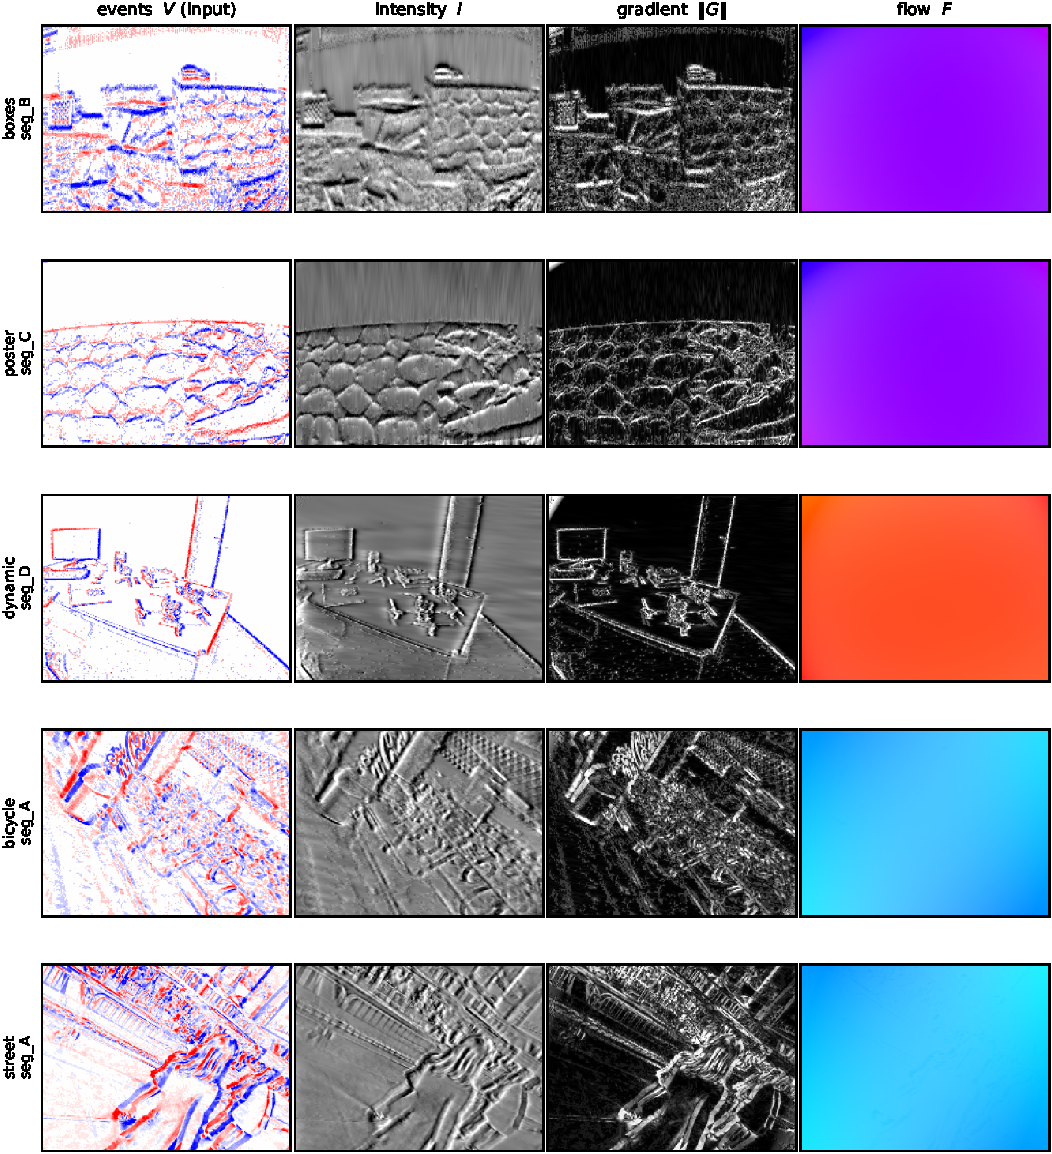
\includegraphics[width=\textwidth]{fig_appendix_maps}
\caption{Inferred quantities for all five sequences after $40$ frames, at the
configuration of Table~\ref{tab:main}. Only $\Vmap$ is observed; $\Imap$,
$\Gmap$ and $\Fmap$ are inferred jointly with $\wvec$. Flow is coded as hue for
direction and saturation for magnitude.}
\label{fig:appendix}
\end{figure*}


\section{Convergence on a Real Sequence}
\label{app:converge}

Figure~\ref{fig:converge_poster} is the counterpart of
Fig.~\ref{fig:converge} on a real sequence. The pattern is the same --- the
sequential scheme has structure after one iteration, the simultaneous ones by
about ten --- but here the sequential scheme does not diverge, so the two end in
comparable states. Together the two figures show that the stability difference
is sequence-dependent while the convergence-rate difference is not.

\begin{figure*}[!t]
\centering
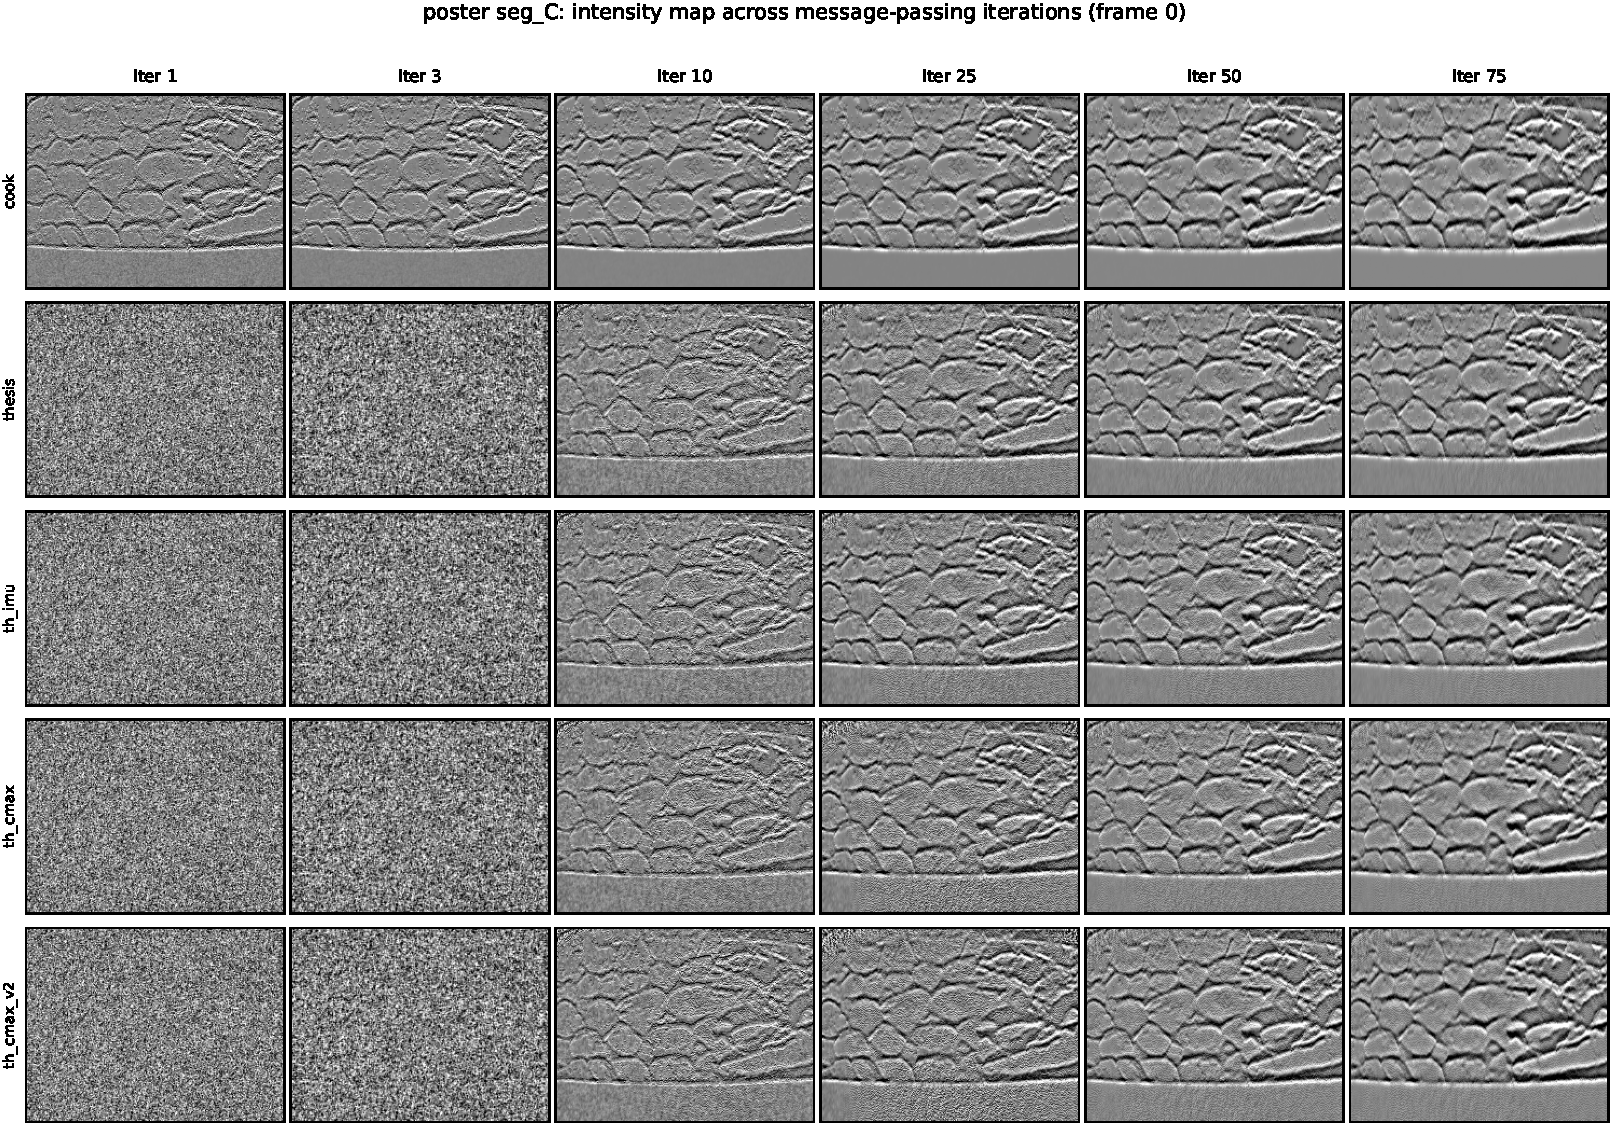
\includegraphics[width=\textwidth]{fig_converge_poster}
\caption{Intensity map across the iterations of a single frame
(\texttt{poster}, first frame), for all five models, initialised from noise at
that frame as in Fig.~\ref{fig:converge}.}
\label{fig:converge_poster}
\end{figure*}


\section*{Acknowledgment}
The authors would like to thank Prof.\ Guillermo Gallego for supervising this
project.


\begin{thebibliography}{99}

\bibitem{lichtsteiner2008}
P.~Lichtsteiner, C.~Posch, and T.~Delbruck, ``A 128$\times$128 120\,dB
15\,$\mu$s latency asynchronous temporal contrast vision sensor,''
\emph{IEEE J. Solid-State Circuits}, vol.~43, no.~2, pp. 566--576, 2008.

\bibitem{gallego2022survey}
G.~Gallego, T.~Delbr\"uck, G.~Orchard, C.~Bartolozzi, B.~Taba, A.~Censi,
S.~Leutenegger, A.~J. Davison, J.~Conradt, K.~Daniilidis, and D.~Scaramuzza,
``Event-based vision: A survey,'' \emph{IEEE Trans. Pattern Anal. Mach.
Intell.}, vol.~44, no.~1, pp. 154--180, 2022.

\bibitem{cook2011}
M.~Cook, L.~Gugelmann, F.~Jug, C.~Krautz, and A.~Steger, ``Interacting maps for
fast visual interpretation,'' in \emph{Proc. Int. Joint Conf. Neural Networks
(IJCNN)}, 2011, pp. 770--776.

\bibitem{martel2019thesis}
J.~N.~P. Martel, ``Unconventional processing with unconventional visual sensing:
Parallel, distributed and event based vision algorithms \& systems,'' Ph.D.
dissertation, ETH Z\"urich, 2019.

\bibitem{martel2015relational}
J.~N.~P. Martel and M.~Cook, ``A framework of relational networks to build
systems with sensors able to perform the joint approximate inference of
quantities,'' in \emph{IROS Workshop on Advances in Biologically Inspired
Brain-Like Cognition and Control for Learning Robots}, 2015.

\bibitem{kschischang2001}
F.~R. Kschischang, B.~J. Frey, and H.-A. Loeliger, ``Factor graphs and the
sum-product algorithm,'' \emph{IEEE Trans. Information Theory}, vol.~47, no.~2,
pp. 498--519, 2001.

\bibitem{horn1981}
B.~K.~P. Horn and B.~G. Schunck, ``Determining optical flow,'' \emph{Artificial
Intelligence}, vol.~17, no.~1--3, pp. 185--203, 1981.

\bibitem{kim2014}
H.~Kim, A.~Handa, R.~Benosman, S.-H. Ieng, and A.~J. Davison, ``Simultaneous
mosaicing and tracking with an event camera,'' in \emph{Proc. British Machine
Vision Conf. (BMVC)}, 2014.

\bibitem{gallego2018cmax}
G.~Gallego, H.~Rebecq, and D.~Scaramuzza, ``A unifying contrast maximization
framework for event cameras, with applications to motion, depth and optical flow
estimation,'' in \emph{Proc. IEEE Conf. Computer Vision and Pattern Recognition
(CVPR)}, 2018, pp. 3867--3876.

\bibitem{mueggler2017}
E.~Mueggler, H.~Rebecq, G.~Gallego, T.~Delbruck, and D.~Scaramuzza, ``The
event-camera dataset and simulator: Event-based data for pose estimation, visual
odometry, and SLAM,'' \emph{Int. J. Robotics Research}, vol.~36, no.~2, pp.
142--149, 2017.

\bibitem{guo2024cmaxslam}
S.~Guo and G.~Gallego, ``CMax-SLAM: Event-based rotational-motion bundle
adjustment and SLAM system using contrast maximization,'' \emph{IEEE Trans.
Robotics}, vol.~40, 2024.

\end{thebibliography}

\end{document}
